\documentclass{article}
\usepackage{neurips_2026}
\usepackage[utf8]{inputenc}
\usepackage[T1]{fontenc}
\usepackage[hidelinks]{hyperref}
\usepackage{url}
\usepackage{booktabs}
\usepackage{amsfonts,amsmath,amssymb,amsthm}
\usepackage{nicefrac}
\usepackage{microtype}
\usepackage{xcolor}
\usepackage{graphicx}
\usepackage{array}

\newtheorem{proposition}{Proposition}
\newtheorem{lemma}{Lemma}
\newtheorem{conjecture}{Conjecture}

\title{Which Benchmarks, and How Many? Cold-Start Benchmark Selection as Experimental Design on Leaderboard Score Matrices}
\author{Anonymous authors}

\begin{document}
\maketitle

\begin{abstract}
A new model can be run on only $k$ of $N$ benchmarks: which $k$, how should the other scores be inferred, and how large must $k$ be?
We treat this cold-start problem as Bayesian experimental design on a latent-factor model of the leaderboard score matrix, evaluated under a leakage-safe protocol for sparse, non-stationary leaderboards, with a floor on the error of every selector, a finite-history correction, and two stopping rules.
We test the theory on synthetic matrices with known truth and the selection on MTEB and on generative-LLM leaderboards.
On the complete MTEB block of 103 models and 202 tasks, three benchmarks chosen by the model reduce the error from 1.03 to 0.60 standard deviations, 28\% in MSE below three random ones; but an error of 0.5 takes 20 chosen or 60 random benchmarks, and recovering the ten best history models reaches an F1 of only 0.74 at $k=60$.
The closed-form forecast is accurate with known parameters and optimistic by 10--20\% when fitted on real data; the factor posterior is 22\% less accurate than ExtraTrees at the same selected set, yet the gain from selection survives the change of imputer.
Under temporal shift the nominal 90\% intervals cover 76--80\% of scores on MTEB.
On five generative-LLM leaderboards (6 to 57 benchmarks) the A-optimal criterion beats random choice at the smallest budgets and not at the largest, where the complement-error greedy is never worse; with whole organisations held out the gain at $k=3$ holds on MTEB-A1 and the sparse matrix but not on MTEB-A2, where one organisation carries most of the error, and the advantage at large $k$ does not hold on the sparse matrix.

\end{abstract}

\section{Introduction}
\label{sec:intro}
Evaluating a model on a benchmark suite is expensive, and public leaderboards already hold the scores of hundreds of models on dozens or hundreds of benchmarks.
An evaluator with a new model and room for only $k$ benchmark runs faces three questions: which $k$ benchmarks to run, how to infer the scores on the other $N-k$, and how large $k$ must be before the inference is good enough.
Existing work shrinks the items inside one benchmark \citep{polo2024tinybenchmarks,vivek2024anchor,kipnis2024metabench}, measures how benchmarks agree \citep{perlitz2024benchbench}, or predicts scores from scale and model family \citep{ruan2024observational,polo2024sloth}; to our reading, none of them asks which whole benchmarks to run on a new model, nor how many.

We study this cold-start problem on the leaderboard score matrix itself.
Our reading of it is Bayesian experimental design on a latent-factor model: the posterior of a few latent capabilities given the $k$ scores run gives the prediction, a closed-form greedy gain chooses the benchmarks, and the posterior covariance forecasts the error and yields a stopping rule for $k$.
Gaussian sensor placement and the factor algebra are standard \citep{krause2008nearoptimal,das2011submodular}; we claim none of it as new.
The contribution is the combination with a protocol and with evidence that shows where it holds and where it does not.

\begin{figure}[t]
\centering
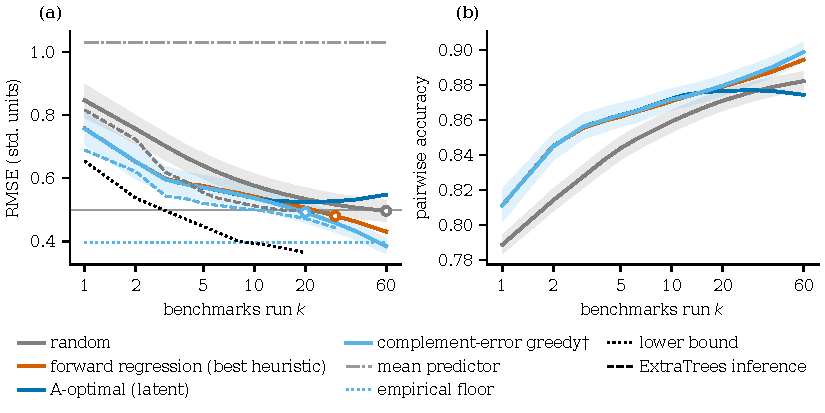
\includegraphics[width=\textwidth]{figures/f1.pdf}
\caption{A few benchmarks remove most of the error, but a tight tolerance needs many more. MTEB block A1 (103 models, 202 benchmarks), factor-posterior inference. (a) RMSE in standard-deviation units against the number of benchmarks run $k$: random choice, the A-optimal criterion, the complement-error greedy$^\dagger$ ($^\dagger$: added after a pilot) and forward regression, the best heuristic; bands: 95\% intervals; dashed: the same random and complement-error selections with ExtraTrees inference (no such curve in (b)); open circles mark the first grid $k$ with RMSE $\le0.5$. Dotted: the lower bound of Proposition~\ref{prop:floor} and the empirical floor (each benchmark predicted from all others), references not bounds. (b) Pairwise accuracy of ``which history models does the new model beat''.}
\label{fig:f1}
\end{figure}

\paragraph{Contributions.}
\begin{itemize}
\item \emph{A protocol} for sparse, non-stationary leaderboards in which every fitted quantity uses history rows only, a test model is scored on benchmarks it has actually been run on, and random, temporal and family-held-out splits are compared (Section~\ref{sec:setting}).
\item \emph{Theory with its checks.} An error decomposition, a floor on the error of every selector, a water-filling law for the achievable curve, and a conjecture for the effect of finite history from spiked-covariance theory, tested on synthetic matrices where the truth is known and on real ones; the closed-form forecast is accurate with known parameters and optimistic when fitted, and our finite-history correction does not improve on the plug-in forecast (Sections~\ref{sec:theory}, \ref{sec:experiments}).
\item \emph{An empirical map} of when few benchmarks suffice, with decision metrics beside RMSE, nonlinear imputers as the accuracy reference, and the effect of temporal and family shift.
\end{itemize}

\paragraph{What we find.}
On the complete MTEB block (103 models, 202 tasks), three benchmarks chosen by the model cut the RMSE from 1.03 (the history mean) to 0.60 standard deviations, $28\%$ below the MSE of three random ones (Figure~\ref{fig:f1}).
But the curve then flattens: an RMSE of 0.5 needs 20 benchmarks chosen by the best selector and 60 chosen at random.
The closed-form error is accurate when the factor model is known (97\% of synthetic cells within 10\%) but optimistic by 10--20\% when it is fitted, and a nonlinear imputer is 22\% more accurate than the factor model at the same selected set, although the advantage of selection over random choice holds under either.
Section~\ref{sec:experiments} gives the full map, including shift and what the generative-LLM leaderboards, with at most 57 benchmarks, can and cannot show.

\section{Related work}
\label{sec:related}
\paragraph{Fewer items inside one benchmark.}
tinyBenchmarks, anchor points, metabench and later work shrink the item set of a benchmark and estimate that benchmark's score from the retained items \citep{polo2024tinybenchmarks,vivek2024anchor,kipnis2024metabench,perlitz2024efficient,hofmann2025fluid,yauney2025reliable}.
Their unit of cost is an item; ours is a whole benchmark, and the quantity to infer is the score on the \emph{other} benchmarks.
\paragraph{Agreement and low-dimensional predictors.}
BenchBench quantifies how benchmarks agree \citep{perlitz2024benchbench}; observational scaling laws, Sloth and a latent-variable scaling law predict benchmark scores through a few capability factors estimated from many public models, from model features rather than from benchmarks already run \citep{ruan2024observational,polo2024sloth,cai2025latent}.
Factor analyses of language-model scores find a few broad abilities \citep{burnell2023revealing,ilic2023evidence}; Burnell et al.\ suggest that benchmarks could be streamlined to one task per ability.
We take that low-dimensional structure as our premise and turn it into a selection of benchmarks, a held-out prediction and a derived number $k$ to run.
\paragraph{Item response theory and adaptive testing.}
Psychometric adaptive testing selects items by their information about a latent ability \citep{segall1996multidimensional}, and item response models have been used to build NLP evaluation scales, compare test sets and reweight evaluation examples \citep{lalor2016building,vania2021comparing,rodriguez2021evaluation,lalor2024irt}; recent work argues for the same approach for language models and applies Fisher-information item selection inside one benchmark \citep{zhuang2023position,li2025atlas}.
Their unit is again the item and the target is the ability or the score of the benchmark it comes from; we choose among whole benchmarks, with their unequal cost, to predict the scores on those not run.
\paragraph{Cold-start elicitation and experimental design.}
Choosing which items a new user should rate has the structure of our problem \citep{golbandi2011adaptive,elahi2016survey}; the machinery for choosing observations in a Gaussian model is greedy sensor placement with submodularity guarantees \citep{krause2005nonmyopic,krause2008nearoptimal}, and for variance reduction the submodularity ratio of \citet{das2011submodular}, see also \citet{khanna2017scalable}.
Column subset selection and leverage scores choose representative columns \citep{cohen2017input}; matrix completion recovers entries observed at random \citep{candes2009exact,mazumder2010spectral}, whereas here the observed set is chosen, budgeted, and lies in a new row.
We use this machinery and claim no novelty for it.

\section{Setting and evaluation protocol}
\label{sec:setting}
\paragraph{Problem.}
A history of $M$ models has been scored on $N$ benchmarks; the score matrix $X\in\mathbb{R}^{M\times N}$ may have missing cells (mask $\Omega$).
A new model can be run on $k$ benchmarks $S$ chosen from those it can be run on, and the evaluator wants its scores on the other benchmarks $T$.
We call $k^\ast(\epsilon)$ the smallest $k$ at which the error on $T$ falls to a tolerance $\epsilon$.
Scores are standardised per benchmark with the mean and standard deviation of the history rows only, so that errors are in units of a benchmark's standard deviation and benchmarks on different scales (accuracy, win rate, nDCG) are comparable.

\paragraph{Protocol.}
The unit of replication is the held-out \emph{model}.
The models are split into history and test models by repeated 5-fold partitions; for every split, the standardisation, the factor model and its rank, all hyper-parameters (chosen by cross-validation inside the history), the selection order, and the conformal calibration use history rows only.
A test model is scored on a benchmark only if it has a score there: on sparse matrices the candidates for $S$ are the test model's own observed benchmarks and $T$ is its remaining observed benchmarks, so no score is ever imputed for evaluation.
Confidence intervals are 95\% percentile bootstrap intervals over held-out models, after averaging over repeated splits (and over random draws for the random selector).
We report, at each $k$: RMSE in standardised units over $T$; the pairwise accuracy of the question ``which history models does the new model beat'' on each target, averaged over targets; top-10 F1 (does the predicted ranking recover the history models in the top ten); and Spearman correlation across a model's targets.
Fitting on all rows, with the test models in the history, makes the error look smaller by $0.04$--$0.10$ in MSE ($10$--$23\%$ in RMSE) on MTEB, with 95\% intervals that exclude zero in every cell (Appendix~\ref{app:protocol}).

\paragraph{Matrices.}
Table~\ref{tab:t1} (Appendix~\ref{app:data}) lists the matrices.
The primary data are the MTEB text-embedding leaderboard results \citep{muennighoff2022mteb} at a pinned commit (CC0-1.0): the ``models'' are embedding models and the ``benchmarks'' are embedding tasks, not generative LLMs.
Two settings are fixed from the missingness pattern alone, before any error was computed: a complete block of 103 models $\times$ 202 tasks, found by repeatedly dropping the lowest-coverage row or column (A1), and the 126 models complete on the 30 most-covered tasks (A2); and the sparse matrix of 507 models $\times$ 598 tasks with 22\% of cells observed, with the availability constraint above (B).
As a second kind of matrix we use generative-LLM leaderboards (Open LLM Leaderboard v2 \citep{fourrier2024open}, HELM Lite and HELM MMLU \citep{liang2022helm}, LiveBench \citep{white2024livebench}) with $N$ between 6 and 57; for these, held-out folds are whole model families or organisations.
Synthetic matrices with known loadings serve to check the theory (Section~\ref{sec:theory}).

\paragraph{Comparisons.}
The confirmatory comparisons were written down before the confirmatory runs (budgets $k\in\{3,8,20\}$): the greedy selector against random choice and against clustering, pivoted-QR, leverage-score and centrality selectors; the factor posterior against ridge, kNN and softImpute \citep{mazumder2010spectral}; cost-aware against cost-ignorant selection; conformal against model-based stopping.
They are Holm-corrected \citep{holm1979simple} as one family per experiment and matrix; everything else is labelled exploratory.
Two comparisons were added after a pilot on a separate seed had shown that the first criterion degrades at large $k$ (Section~\ref{sec:experiments}); they are marked $\dagger$.

\section{Method}
\label{sec:method}
\paragraph{Inference.}
We model standardised scores of a model as $x=\mu+\Lambda z+\varepsilon$ with $z\sim\mathcal N(0,I_r)$ and $\varepsilon\sim\mathcal N(0,\Psi)$, $\Psi=\mathrm{diag}(\psi_j)$ (factor analysis).
$\mu,\Lambda,\Psi$ are fitted by EM on the history, with missing cells handled by the marginal likelihood of the observed entries and a floor on $\psi_j$; the rank $r$ is chosen by held-out likelihood on history models.
Given the scores $x_S$ of the $k$ benchmarks run, the posterior of the latent profile is Gaussian with covariance $P_S=(I+\Lambda_S^\top\Psi_S^{-1}\Lambda_S)^{-1}$, the prediction for each target is $\hat x_j=\mu_j+\lambda_j^\top \mathbb{E}[z\mid x_S]$, and its predictive variance is $\psi_j+\lambda_j^\top P_S\lambda_j$.
The model is an assumption; we measure rather than assume its rank, and compare its accuracy with nonlinear imputers (Section~\ref{sec:experiments}).

\paragraph{Selection.}
Choosing $S$ is Bayesian experimental design on this model.
Because $P_S^{-1}=I+\sum_{j\in S}\lambda_j\lambda_j^\top/\psi_j$, adding benchmark $j$ to $S$ changes $P$ by a rank-one update, and the gain in the latent variance reduction $f_W(S)=\mathrm{tr}\,W(I-P_S)$ is in closed form,
\begin{equation}
\Delta_j(S)=\frac{\lambda_j^\top P_S W P_S\lambda_j}{\psi_j+\lambda_j^\top P_S\lambda_j},\qquad P_{S+j}=P_S-\frac{P_S\lambda_j\lambda_j^\top P_S}{\psi_j+\lambda_j^\top P_S\lambda_j},
\label{eq:gain}
\end{equation}
so a greedy step costs $O(Nr^2)$.
We use three weights: $W=\Lambda^\top\Lambda$ (all latent directions matter; \emph{A-optimal}); $W=\Lambda_T^\top\Lambda_T$ for a fixed target group $T$ (\emph{target-aware}, for transfer to a group of tasks not run); and the criterion that minimises the expected squared error on the complement of the selected set, in which the selected benchmarks leave the target set (\emph{complement-error}). 
A cost-aware variant (gain per unit of measured evaluation time) and a rank-free variant that conditions an empirical shrunk covariance directly complete the family.
The baselines are random choice, most-covered, centrality, k-medoids clustering of $|{\rm corr}|$, pivoted QR, leverage scores and greedy forward regression, all fitted on history rows.

\paragraph{Forecast and stopping.}
The posterior variance forecasts the error of a selection from the history fit alone, $\mathrm{MSE}(S)=\frac1{|T|}\bigl(\sum_{j\in T}\psi_j+\mathrm{tr}(\Lambda_T^\top\Lambda_T P_S)\bigr)$, with the finite-history correction of Section~\ref{sec:theory}.
Two stopping rules choose $k$: the \emph{model-based} rule takes the smallest $k$ at which the forecast RMSE is $\le\epsilon$; the \emph{split-conformal} rule \citep{lei2018distribution} takes the smallest $k$ at which the mean (or the 90\% quantile) of leave-one-model-out RMSE over history models is $\le\epsilon$, which needs no model assumption but assumes the new model resembles the history.

\paragraph{Applicability and cost.}
Computation is small next to running a benchmark; the cost that matters is the history, which must be large enough to resolve factors whose signal-to-noise is above $\sqrt{N/M}$ (Section~\ref{sec:theory}) and must contain the benchmark: one not in the history cannot be chosen or predicted.

\section{Theory: how the error depends on $k$}
\label{sec:theory}
All statements are for the model of Section~\ref{sec:method} with known parameters unless said otherwise; proofs are in Appendix~\ref{app:proofs}.
$W_T=\Lambda_T^\top\Lambda_T$ with eigenvalues $\lambda_1(W_T)\ge\lambda_2(W_T)\ge\dots$

\begin{proposition}[Error of a selection]\label{prop:decomp}
For a fixed $S$ and targets $T$, the Bayes predictor has expected squared error summed over $T$ equal to $\sum_{j\in T}\psi_j+\mathrm{tr}(W_TP_S)$. $P_S$ does not depend on the observed values, so an adaptive policy that picks the next benchmark after seeing scores cannot beat the best fixed set of size $k$.
\end{proposition}
Both statements are textbook Gaussian algebra; we state them because Section~\ref{sec:experiments} uses them: the first as the forecast, the second to read any gain of an adaptive policy on real data as a sign of non-Gaussian structure.

\begin{proposition}[A floor for every selector]\label{prop:floor}
For every $S$ with $|S|=k$ and every fixed $T$, $\mathrm{tr}(W_TP_S)\ge\sum_{i>k}\lambda_i(W_T)$. Hence $\mathrm{error}(k)\ge\sum_{j\in T}\psi_j+\sum_{i>k}\lambda_i(W_T)$.
\end{proposition}
The floor needs no assumption on the spectrum: a sharp knee at the rank is only one case.
It ignores noise in the observed scores and is therefore a floor, not a forecast; we draw it as a sanity reference.
When $T$ is the complement of $S$ the same argument holds with $\lambda_i(W_T)\ge\lambda_{i+k}(\Lambda^\top\Lambda)$ (Weyl), i.e.\ the tail of $\Lambda^\top\Lambda$ beyond $2k$.

\paragraph{Where the curve goes.}
If every benchmark loads on one of $r$ orthogonal factors, the latent error is $\sum_i W_{ii}/(1+k_i\rho_i)$ with $k_i$ benchmarks on factor $i$ and $\rho_i=\lambda_i^2/\psi$, and the best split of $k$ over factors is reverse water-filling (Appendix~\ref{app:proofs}): factors with large $W_{ii}$ get benchmarks first.
For balanced factors the error reaches a tolerance when $k\approx r\,(\psi/\lambda^2)(1/\delta-1)$; for a power-law spectrum there is no plateau, and $k^\ast$ grows with the number of factors above the noise.
The plug-in forecast of Section~\ref{sec:method} evaluates the curve with the fitted $(\Lambda,\Psi)$.

\paragraph{Finite history.}
The fitted $\Lambda$ comes from $M$ models, which matters when $N/M$ is not small.
For a factor with signal-to-noise $\rho_i=\|\lambda_i\|^2/\bar\psi$, spiked-covariance theory \citep{baik2005phase,baik2006eigenvalues,paul2007asymptotics} says that the sample covariance recovers its direction only if $\rho_i>\sqrt{N/M}$, with squared overlap $(1-c/\rho_i^2)/(1+c/\rho_i)$, $c=N/M$.
\begin{conjecture}[Finite-history error]\label{conj:fm}
Factors with $\rho_i\le\sqrt{N/M}$ cannot be recovered from $M$ models and add their full variance to $\mathrm{error}(k)$ for every selector and every $k$; factors above the threshold are recovered with shrunk loadings. Hence the effective rank at history size $M$ is $r_{\rm eff}(M)=\#\{i:\rho_i>\sqrt{N/M}\}$, and a forecast built from the fitted model alone is optimistic unless the fitted spikes are de-biased and unrecoverable factors are folded into the noise.
\end{conjecture}
This is a conjecture because the spiked-model results are asymptotic and for isotropic noise, and our noise is heterogeneous; we do not prove it, we test it by simulation (Section~\ref{sec:experiments}).
Our forecast inverts the sample-spike inflation, moves unrecoverable factors into $\Psi$, and multiplies the reducible part of the error by $1+k_{\rm eff}/(M-k_{\rm eff}-1)$, the classical finite-sample inflation of least squares with $k_{\rm eff}=\min(k,r_{\rm eff})$ regressors.

\paragraph{Greedy versus optimal.}
For the all-latent weight or a fixed target set, $f_W(S)=\mathrm{tr}\,W(I-P_S)$ is monotone and has a submodularity ratio $\gamma>0$ in the sense of \citet{das2011submodular}, so greedy achieves at least $1-e^{-\gamma}$ of the optimum; this holds for the A-optimal and target-aware criteria but not for the complement-error criterion, whose target set moves with $S$, so for the latter greedy is only compared empirically with a local-search optimum (Appendix~\ref{app:greedy}).
On A1 and A2 greedy reaches at least $94.7\%$ of the best $f_W$ found by exhaustive or local search; the guarantee itself is vacuous there, since the estimated $\gamma$ is $0.01$--$0.02$.

\section{Experiments}
\label{sec:experiments}
Errors are RMSE in standardised units over the targets of a held-out model, with 95\% bootstrap intervals over held-out models (Section~\ref{sec:setting}); on MTEB-A1 and A2 each cell is the mean of 10 repetitions of 5-fold splits, and random selection averages at least 100 draws.
Inference is the factor posterior unless stated; the matrices are listed in Table~\ref{tab:t1} (Appendix~\ref{app:data}).
The selectors are the A-optimal criterion on the latent factors (the declared one) and the complement-error greedy$^\dagger$, added after a pilot on a separate seed had shown the A-optimal criterion degrading at large $k$.


\subsection{How fast the error falls with $k$}
Figure~\ref{fig:f1} answers the question on the complete MTEB block A1.
With no benchmark run, the history-mean predictor has RMSE $1.03$.
Running three of the 202 benchmarks, chosen by the A-optimal criterion, brings it to $0.595$ [0.554, 0.637], against $0.701$ [0.657, 0.742] for three random ones; the gain over random is $28\%$ in MSE at $k=3$, $15\%$ at $k=8$ and $3\%$ at $k=20$ (Table~\ref{tab:t2}, all Holm-significant).
After the first few benchmarks the curve flattens: from $k=8$ to $k=20$ the best selector moves from $0.55$ to $0.49$, and an RMSE of $0.5$ is reached at $k=20$ by the complement-error greedy, at $k=60$ by random choice, and never by the A-optimal criterion, whose error rises again after $k\approx15$.
With ExtraTrees inference both selections are lower at small $k$ and the gap between them narrows to $0.017$ in RMSE at $k=8$ ($0.506$ against $0.523$) and $0.011$ at $k=12$ (dashed curves): the advantage of selection does not depend on the factor model, but beyond $k\approx10$ it is small on A1 under any imputer.
The decision metrics move more slowly: for the complement-error greedy the pairwise accuracy of ``which history models does the new model beat'' is $0.856$ at $k=3$ and $0.899$ at $k=60$ (random: $0.828$, $0.882$), and the top-10 F1 $0.61$ and $0.74$.

\subsection{Does the theory predict the curve?}
Figure~\ref{fig:f2} separates the two questions.
Where the truth is known (synthetic matrices with $N=48$, three spectra, $M\in\{30,60,125,500\}$, three signal-to-noise levels, 252 cells), the closed form of Proposition~\ref{prop:decomp} with the true parameters stays within 10\% of the measured error in 97\% of cells (median gap 1.8\%), meeting the pre-declared threshold of 90\%.
With parameters fitted from $M$ models it does not: the plug-in forecast stays within 10\% in 72\% of cells and the finite-history forecast in 73\%, so the correction of Section~\ref{sec:theory} does not improve on the plug-in; both fail the threshold at $M=30$ and $M=60$ (27\%, and 62\% and 65\% of cells within 10\%) and pass it at $M\ge125$ (98--100\%).
The effective-rank prediction of Conjecture~\ref{conj:fm} holds in 27 of 36 cells (rank chosen by held-out likelihood within 2 of $r_{\rm eff}(M)$); eight of the nine misses are the power-law spectrum with $M<500$, so we read the conjecture as supported for block spectra and an over-estimate for slowly decaying ones.

On the real matrices the forecast built from the history fit alone is optimistic.
On A1 its signed error in RMSE is $-10\%$ at $k=1$ and $-19\%$ at $k=20$, on A2 $-6\%$ and $-20\%$; the median gap is $15\%$ (A1) and $11\%$ (A2), within the 20\% tolerance we had set for real matrices and outside the 10\% we had set for synthetic ones from $k=3$ on.
The rank chosen by held-out likelihood is within 2 of the predicted effective rank in every fold (A1: 8.3 against 8.3; A2: 4.8 against 4.7).
Varying the history size shows where this stops holding: the forecast is optimistic at every $M$ on MTEB and the rank is resolved only when the history is nearly the whole matrix, whereas on the Open LLM Leaderboard matrices ($M$ up to $2000$) the gap is at most $3.4\%$ from $M=500$; the correction helps when $M$ is large against $N$ (Appendix~\ref{app:history}).

\begin{figure}[t]
\centering
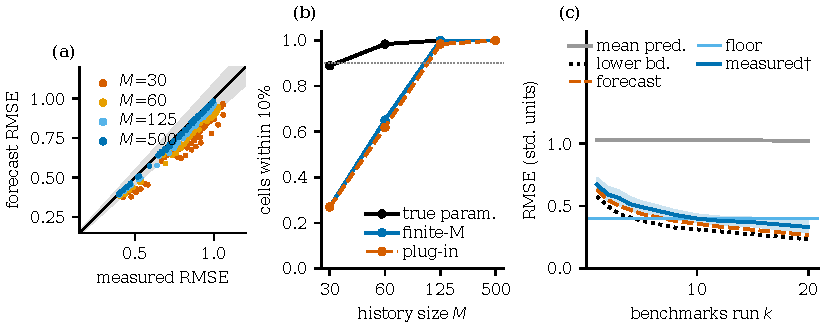
\includegraphics[width=\textwidth]{figures/f2.pdf}
\caption{Forecast against measurement. (a) Synthetic matrices: finite-history forecast against measured RMSE, $\pm10\%$ band, coloured by history size $M$. (b) Share of synthetic cells within 10\% of the measured error for the true parameters, the finite-history forecast and the plug-in forecast. (c) MTEB-A2: the forecast lies below the measured error at every $k$; the grey line is the mean predictor, the lower bound (lower bd.) and the empirical floor are references. The forecast refers to the complement-error greedy$^\dagger$.}
\label{fig:f2}
\end{figure}

\subsection{When selection matters}
Table~\ref{tab:t2} compares selectors and inference methods on the primary family.
With random folds the A-optimal criterion beats random choice at $k=3$ on both MTEB blocks, but not uniformly: on A2 ($N=30$) the gain is not significant at $k=8$ and at $k=20$, two thirds of the benchmarks, it has $52\%$ higher error than random [$+36$, $+72$].
The complement-error greedy$^\dagger$ is better than random at every $k$ of the grid on A1 ($-28$, $-15$, $-15\%$) and A2 ($-20$, $-32$, $-50\%$).
Among the heuristics, pivoted QR, leverage scores and centrality are clearly worse than A-optimal selection on A1 ($-17\%$ to $-61\%$); $k$-medoids clustering is within a few per cent of it and better at $k=20$ on A1 and, markedly, on A2 at $k=8$ and $20$.
A model-free cluster of benchmarks is a strong baseline; the factor model adds the closed-form gain, the forecast, and the target-aware and cost-aware variants of Section~\ref{sec:method}.
In a comparison we added after the pilot and kept outside the declared family, the complement-error greedy$^\dagger$ is never worse than $k$-medoids or forward regression on A1 and A2 but on B it is worse than $k$-medoids at $k=8$ ($+5\%$) and not better than forward regression: simple selectors are competitive there (Appendix~\ref{app:fam}).
On the sparse matrix B (507 models, 598 tasks, 22\% observed; three repetitions) the A-optimal criterion beats random by $22\%$ at $k=3$, ties it at $k=8$ ($-2\%$, not significant) and loses by $14\%$ at $k=20$, where the complement-error greedy$^\dagger$ beats random by $15\%$ and A-optimal by $26\%$ (Appendix~\ref{app:t2full}).
Under folds made of whole organisations, with a bootstrap over organisations (Appendix~\ref{app:fam}), no decision of Table~\ref{tab:t2} changes in the random folds, and the gains at $k=3$ hold on A1 and B ($-27\%$ on A1 and $-12\%$ on B for the complement-error greedy$^\dagger$ against random) and the complement-error greedy stays better than random on A1 at every $k$.
Not all survives: on A2 the gain at $k=3$ does not hold ($-4\%$ for both selectors): one organisation carries most of the error and the A-optimal criterion is no better than random at $k=3$ and $8$ and worse at $k=20$; on B the greedy's gain at $k=20$ is a tie ($+8\%$, n.s.) against $-15\%$.
On the five generative-LLM matrices (five repetitions of family-held-out folds, cluster selection not run; Table~\ref{tab:t3} in Appendix~\ref{app:t2full}) the A-optimal criterion beats random choice at the smallest budgets (HELM Lite $-28\%$ in MSE at $k=2$, HELM MMLU $-25\%$ and the Open LLM Leaderboard subtasks $-23\%$ at $k=3$), and is worse or no better at the largest: $+11\%$ at $k=20$ on HELM MMLU, $+7\%$ at $k=3$ on the six-benchmark Open LLM Leaderboard matrix, no significant difference on LiveBench.
The complement-error greedy$^\dagger$ is never worse than random and is better on HELM Lite, on both Open LLM Leaderboard matrices ($-18\%$ to $-49\%$) and, at $k=3$, on HELM MMLU; on LiveBench (77\% observed) its gain is not significant.

\begin{table}[t]
\centering\scriptsize\setlength{\tabcolsep}{3pt}
\begin{tabular}{@{}lrrr@{}}
\toprule
Comparison & $k=3$ & $k=8$ & $k=20$ \\
\midrule
\multicolumn{4}{@{}l}{\textit{MTEB-A1}} \\
P1 A-optimal vs random & \textbf{$-$28 [$-$33,$-$22]} & \textbf{$-$15 [$-$19,$-$10]} & \textbf{$-$3 [$-$5,$-$2]} \\
P3 A-optimal vs cluster & $+$3 [$-$1,$+$10] & $-$2 [$-$5,$+$1] & \textbf{$+$3 [$+$2,$+$5]} \\
P3 A-optimal vs pivqr & \textbf{$-$42 [$-$48,$-$35]} & \textbf{$-$40 [$-$47,$-$34]} & \textbf{$-$17 [$-$22,$-$12]} \\
P5 FA vs ridge (A-optimal) & 0 [$-$2,$+$2] & $+$2 [$-$1,$+$7] & \textbf{$+$7 [$+$5,$+$9]} \\
P5 FA vs kNN (A-optimal) & $+$9 [$+$2,$+$15] & $+$6 [$-$1,$+$13] & 0 [$-$6,$+$5] \\
P5 FA vs softImpute (A-optimal) & \textbf{$-$21 [$-$28,$-$14]} & \textbf{$-$11 [$-$17,$-$5]} & $+$2 [$-$1,$+$4] \\
P7 complement-error greedy vs A-optimal\,$\dagger$ & 0 & 0 [0,$+$1] & \textbf{$-$12 [$-$16,$-$9]} \\
P7 complement-error greedy vs random\,$\dagger$ & \textbf{$-$28 [$-$33,$-$22]} & \textbf{$-$15 [$-$18,$-$10]} & \textbf{$-$15 [$-$19,$-$12]} \\
\midrule
\multicolumn{4}{@{}l}{\textit{MTEB-A2}} \\
P1 A-optimal vs random & \textbf{$-$20 [$-$25,$-$15]} & $-$3 [$-$9,$+$4] & \textbf{$+$52 [$+$36,$+$72]} \\
P3 A-optimal vs cluster & $+$2 [$-$4,$+$8] & \textbf{$+$16 [$+$8,$+$25]} & \textbf{$+$90 [$+$65,$+$122]} \\
P3 A-optimal vs pivqr & \textbf{$-$23 [$-$34,$-$9]} & $+$17 [$+$2,$+$35] & \textbf{$+$249 [$+$188,$+$324]} \\
P5 FA vs ridge (A-optimal) & 0 [$-$1,$+$1] & \textbf{$+$5 [$+$2,$+$9]} & \textbf{$+$20 [$+$12,$+$31]} \\
P5 FA vs kNN (A-optimal) & \textbf{$+$25 [$+$13,$+$40]} & $+$6 [0,$+$12] & $+$10 [$+$2,$+$18] \\
P5 FA vs softImpute (A-optimal) & \textbf{$-$13 [$-$18,$-$9]} & \textbf{$-$7 [$-$11,$-$2]} & \textbf{$+$11 [$+$7,$+$16]} \\
P7 complement-error greedy vs A-optimal\,$\dagger$ & 0 [$-$3,$+$3] & \textbf{$-$30 [$-$45,$-$17]} & \textbf{$-$67 [$-$88,$-$50]} \\
P7 complement-error greedy vs random\,$\dagger$ & \textbf{$-$20 [$-$24,$-$16]} & \textbf{$-$32 [$-$45,$-$21]} & \textbf{$-$50 [$-$65,$-$37]} \\
\bottomrule
\end{tabular}

\caption{Primary comparisons on MTEB-A1 and A2: relative change in held-out MSE (\%), first named minus second (negative: first is better), with 95\% unadjusted intervals over held-out models; \textbf{bold}: Holm-adjusted $p<0.05$ over the full family of each matrix (P1--P8), of which 8 of the 12 comparisons are shown (the rest: Appendix~\ref{app:t2full}). $\dagger$: added after the pilot. Selectors use factor-posterior inference except where named.}
\label{tab:t2}
\end{table}

\subsection{Groups of tasks and unequal costs}
Two variants of Section~\ref{sec:method} change the question (details and Figure~\ref{fig:f3} in Appendix~\ref{app:groups}).
Choosing benchmarks to predict a group of tasks beats random choice in all ten cells ($12$--$48\%$) but the all-benchmark design in only three ($5$--$12\%$).
Choosing by gain per unit of evaluation time beats the cost-ignorant choice by $44$--$45\%$ on A2 at every budget, where costs are very unequal, but on A1 only at a budget of 5\%.

\subsection{Inference: factor posterior against nonlinear imputers}
Figure~\ref{fig:f6} compares inference methods at the same selected set.
The factor posterior is not the most accurate on MTEB.
At $k=8$ it has $22\%$ (A1) and $25\%$ (A2) higher MSE than ExtraTrees \citep{geurts2006extremely} and $23\%$ (both) than kernel ridge, all Holm-significant; it equals a mixture of factor analysers on A1 ($+0.3\%$) and is $15\%$ worse on A2.
In Table~\ref{tab:t2} it beats softImpute at small $k$ ($-21\%$ at $k=3$ on A1), does not beat ridge or kNN there, and is worse than ridge at $k=20$ on A2 ($+20\%$). On B it beats softImpute at $k=3$ and $8$ ($-22\%$, $-7\%$) and loses to it at $k=20$ ($+10\%$), and is worse than ridge and kNN at every $k$.
On the LLM matrices (Table~\ref{tab:t3}; softImpute not run on the 40-subtask matrix) it beats softImpute everywhere and is indistinguishable from ridge on three of them, but kNN is better on the six-benchmark Open LLM Leaderboard matrix.
What the factor posterior provides in exchange is a predictive variance, hence a forecast of error against $k$ (above), prediction intervals and a stopping rule, which a point-prediction imputer lacks.
The selection gain, however, is not an artefact of the factor model (panels b--d): complement-error selection beats random under all three inference methods at every $k\le20$ on A2 ($-12\%$ to $-51\%$) and under factor analysis and ExtraTrees at every $k\le30$ on A1; under kernel ridge on A1 it helps only at $k=3$ and $8$ and random choice is better at $k=20$ and $30$ ($+17\%$, $+20\%$).
Appendix~\ref{app:rules} compares six inference rules at a fixed selection.

\begin{figure}[t]
\centering
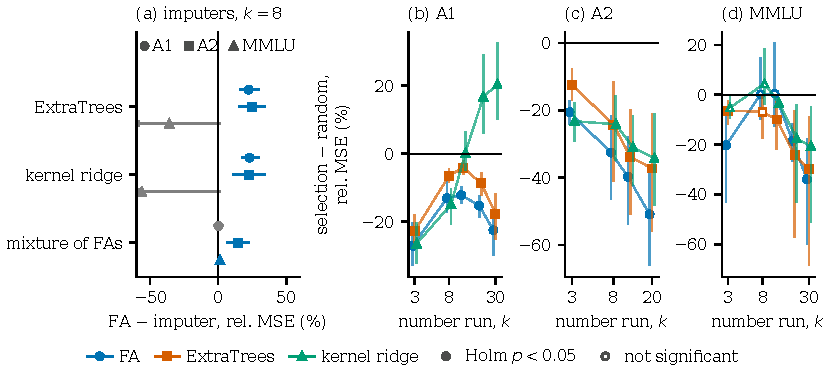
\includegraphics[width=\textwidth]{figures/f6.pdf}
\caption{Inference methods and the selection gain. (a) At the same selected set ($k=8$), FA minus the nonlinear imputer in relative MSE with 95\% intervals; positive means FA is worse; blue: Holm $p<0.05$; arrows: interval cut at the axis. (b--d) A1, A2 and MMLU denote MTEB-A1, MTEB-A2 and HELM MMLU. Complement-error selection minus random choice (relative MSE; negative: selection helps) by inference method; filled: Holm $p<0.05$.}
\label{fig:f6}
\end{figure}

\subsection{Shift}
Under temporal splits (history models are those released earlier) the model-based 90\% intervals cover $0.76$ (A2) and $0.80$ (A1) of the scores on MTEB at $k=3$, and $0.85$ under family-held-out splits; on the LLM matrices coverage is within $0.02$--$0.06$ of nominal (Appendix~\ref{app:shift}).
The error ratio to the mean predictor rises under temporal shift on MTEB (A2 $0.76$ against $0.57$ for random splits), split-conformal coverage stays below $0.90$ ($0.83$, $0.85$), and neither stopping rule is uniformly closer to the measured $k^\ast$.

\subsection{How large must $k$ be?}
We take $k^\ast(\epsilon)$ as the smallest grid $k$ at which the factor-posterior RMSE is at most $\epsilon$ times that of the history-mean predictor, for the complement-error greedy$^\dagger$.
Figure~\ref{fig:f4} places the real matrices on the synthetic grid, whose latent share of variance $h$, history size and spectrum are known.
At $\epsilon=0.7$ one to three benchmarks suffice on every real matrix; at $\epsilon=0.5$ $k^\ast$ is $15$ of $202$ on A1, $5$ of $30$ on A2, $8$ of $40$ on the Open LLM Leaderboard subtasks and $2$ of $57$ on HELM MMLU, while on the sparse matrix B ($h=0.75$) it is not reached within the $20$ benchmarks of the grid (of $598$); the model-based stopping rule would have stopped at $5$ and $3$ on A1 and A2, because its forecast is optimistic.
The latent share alone does not determine $k^\ast$: at $h\approx0.85$ the synthetic $k^\ast$ is $2$ for one factor, $8$--$12$ for four balanced blocks and more than $20$ for a power-law spectrum.
Real matrices with $h$ between $0.75$ and $0.89$ need from $2$ (HELM MMLU) to more than $20$ (B): $k^\ast$ is set by the tolerance and the spectrum, not by $N$.

\begin{figure}[t]
\centering
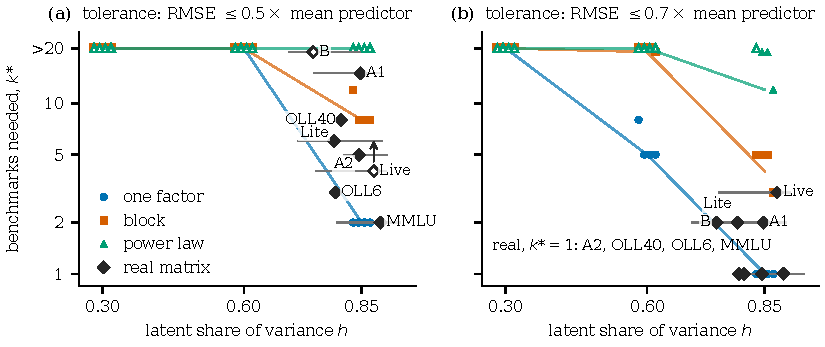
\includegraphics[width=\textwidth]{figures/f4.pdf}
\caption{Benchmarks needed, $k^\ast$, against the latent share of variance $h$. (a) Tolerance: RMSE $\le0.5$ times that of the history-mean predictor; (b) $\le0.7$. Coloured markers: synthetic matrices ($N=48$; one-factor, block and power-law spectra; history sizes $M\in\{30,60,125,500\}$; hollow: not reached by $k=20$), lines: $k^\ast$ from the true parameters. Black diamonds: real matrices at their fitted $h$ (bar: range over folds); hollow: not reached on the grid (arrow where the grid ends below 20). Complement-error greedy$^\dagger$ with factor inference.}
\label{fig:f4}
\end{figure}

\section{Discussion and limitations}
\label{sec:discussion}
\paragraph{What the evidence supports.}
On the embedding leaderboards, a handful of well-chosen benchmarks recovers most of the variance in the other scores, and choosing them with the factor model is worth a quarter of the MSE at $k=3$ against random choice on A1 and (with random folds) A2; the advantage narrows as $k$ grows and depends on the criterion (the A-optimal criterion loses to random choice at large $k$ on A2 and HELM MMLU), the matrix and the imputer.
Small $k$ does not mean exact: a tight tolerance on RMSE, and recovery of the best models among the history, need many more benchmarks than the first factor suggests.

\paragraph{Limits.}
The error forecast is an optimistic reference rather than a calibrated one, and it needs a history several times larger than $N$; the factor model is less accurate than nonlinear imputers on MTEB, so point accuracy calls for pairing the selected set with one, and its intervals need the shift caveat of Figure~\ref{fig:f5}.
Our recommended criterion, the complement-error greedy, was added after a pilot and has no submodularity guarantee; on the sparse matrix B it is not better than $k$-medoids or forward regression, and its gain over random choice at $k=20$ there does not hold for held-out organisations; no stopping rule is validated under shift.
The embedding matrices are one family of leaderboards; the generative-LLM matrices have $N\le57$ benchmarks and mostly two or three factors, too few to carry a $k$-curve, so for them we claim only the comparisons of Section~\ref{sec:experiments}.
Code, pinned data extraction, seeds and result files are supplementary material; licences: Appendix~\ref{app:data}.


\bibliographystyle{plainnat}
{\small\bibliography{references}}

\appendix
\section{Proofs}
\label{app:proofs}
Notation as in Section~\ref{sec:theory}; $Q=\Lambda_S^\top\Psi_S^{-1}\Lambda_S\succeq0$ has rank at most $k=|S|$ and $P_S=(I+Q)^{-1}$.

\paragraph{Proposition~\ref{prop:decomp}.}
Given $x_S$, $z\mid x_S\sim\mathcal N(m_S,P_S)$ where $m_S$ is linear in $x_S$ and $P_S$ does not depend on $x_S$.
For $j\in T$ the Bayes predictor is $\hat x_j=\mu_j+\lambda_j^\top m_S$, and $x_j-\hat x_j=\lambda_j^\top(z-m_S)+\varepsilon_j$ with $\varepsilon_j$ independent of $z-m_S$, so $\mathbb{E}(x_j-\hat x_j)^2=\lambda_j^\top P_S\lambda_j+\psi_j$; summing over $T$ gives $\sum_{T}\psi_j+\mathrm{tr}(W_TP_S)$.
For an adaptive policy the set $S_\tau$ after $\tau$ steps is a function of earlier scores; its final error is $\mathbb{E}[\mathrm{err}(S_k)]$ with $\mathrm{err}(S)$ the above, which depends on $S$ only, so $\mathbb{E}[\mathrm{err}(S_k)]\ge\min_{|S|=k}\mathrm{err}(S)$. (For targets that are the complement of $S$ the same argument applies, with $T=T(S)$.) \qed

\paragraph{Proposition~\ref{prop:floor}.}
$P_S$ and $Q$ commute and share eigenvectors. Let $\Pi$ be the orthogonal projector on $\mathrm{range}(Q)$, $\mathrm{rank}\,\Pi\le k$. On $\mathrm{range}(Q)^\perp$, $P_S$ is the identity; on $\mathrm{range}(Q)$ it is positive semidefinite. Hence $P_S\succeq I-\Pi$ and $\mathrm{tr}(W_TP_S)\ge\mathrm{tr}(W_T)-\mathrm{tr}(W_T\Pi)$.
By Ky Fan's inequality $\mathrm{tr}(W_T\Pi)\le\sum_{i\le k}\lambda_i(W_T)$, and $\mathrm{tr}\,W_T=\sum_i\lambda_i(W_T)$, so $\mathrm{tr}(W_TP_S)\ge\sum_{i>k}\lambda_i(W_T)$. For the complement $T=T(S)$, $W_T=\Lambda^\top\Lambda-\Lambda_S^\top\Lambda_S$ is a perturbation by a PSD matrix of rank $\le k$, so $\lambda_i(W_T)\ge\lambda_{i+k}(\Lambda^\top\Lambda)$ (Weyl). \qed

\paragraph{Block case and water-filling.}
Let each benchmark load on exactly one factor, $\lambda_j=\ell_j e_{i(j)}$, and let $S$ contain $k_i$ benchmarks of factor $i$ with signal-to-noise $\rho_{ij}=\ell_j^2/\psi_j$. Then $Q$ is diagonal with entries $q_i=\sum_{j\in S,i(j)=i}\rho_{ij}$, $P_S=\mathrm{diag}(1/(1+q_i))$ and $\mathrm{tr}(W_TP_S)=\sum_iW_{ii}/(1+q_i)$. With equal $\rho_{ij}=\rho_i$, $q_i=k_i\rho_i$. Minimising over integers $k_i$ with $\sum k_i=k$ is a separable convex problem whose continuous relaxation is solved by reverse water-filling, $1+k_i\rho_i=\sqrt{W_{ii}\rho_i/\nu}$ for a multiplier $\nu$, truncated at $k_i=0$. For $r$ balanced factors ($W_{ii}=W$, $\rho_i=\rho$) the error on the latent part equals $W r/(1+k\rho/r)$, and the latent error reaches a fraction $\delta$ of its initial value $Wr$ at $k=r(1/\delta-1)/\rho$. \qed

\paragraph{Greedy guarantee.}
\label{app:greedy}
Write $f_W(S)=\mathrm{tr}\,W(I-P_S)=\sum_tw_t\mathrm{Var}(s_t)R^2_t(S)$ for $W=\sum_tw_tu_tu_t^\top$, $s_t=u_t^\top z$ and $R^2_t(S)$ the squared multiple correlation of $s_t$ with $x_S$. This is a non-negative combination of variance-explained functions whose submodularity ratio is bounded below by the smallest eigenvalue of the correlation matrix of the observed scores restricted to subsets of bounded size \citep{das2011submodular}; the ratio of a non-negative combination is at least the smallest ratio of its terms, so greedy maximisation of $f_W$ is within $1-e^{-\gamma}$ of the optimum for a fixed $W$. The complement-error criterion is not of this form, because $T$ moves with $S$.

\paragraph{Greedy against the best set found.}
For the fitted factor model of each fold of the first repetition, $f_W$ of the greedy set is compared with that of the best set found for the all-latent weight: by exhaustive search for $k\le4$ ($k\le3$ on A1) and by swap local search started from the greedy set for larger $k$, so for $k\ge4$ the comparison set is the best found, not a certified optimum. The median ratio is $0.948$ ($k=2$), $0.986$, $0.988$, $0.992$ ($k=8$) and $0.997$ ($k=12$) on A1, with minimum $0.947$ over folds and $k$, and $0.975$, $0.983$, $0.998$, $0.999$, $1.000$ on A2 with minimum $0.965$. The complement error of the greedy set is at most $13\%$ above that of the best set found. The estimated submodularity ratio is $\gamma\approx0.010$--$0.024$ for $k\ge2$ ($0.98$ at $k=1$), so $1-e^{-\gamma}\approx0.01$--$0.02$. The sets chosen differ between folds on A1 (mean pairwise Jaccard $0.12$--$0.16$; A2 $0.30$--$0.61$) while their objective values are near-optimal, so the optimum is flat there and individual selected benchmarks should not be interpreted.

\section{Data}
\label{app:data}
\begin{table}[h]
\centering\scriptsize\setlength{\tabcolsep}{3pt}
\begin{tabular}{@{}lrrrrrrrl@{}}
\toprule
Matrix & $M$ & $N$ & density & top-eig. share & part. ratio & FA rank & $h$ & version \\
\midrule
MTEB-A1 & 103 & 202 & 1.00 & 0.57 & 2.9 & 8 & 0.85 & 6dabbcc68c28 \\
MTEB-A2 & 126 & 30 & 1.00 & 0.67 & 2.1 & 4 & 0.84 & 6dabbcc68c28 \\
MTEB-B & 507 & 598 & 0.22 & 0.28 & 9.5 & 2 & 0.75 & 6dabbcc68c28 \\
OLLB v2 (40 subtasks) & 4508 & 40 & 1.00 & 0.61 & 2.6 & 8 & 0.81 & aa81ecc38fdc \\
OLLB v2 (6 benchmarks) & 4576 & 6 & 1.00 & 0.73 & 1.8 & 3 & 0.79 & 9c09a7cae433 \\
HELM MMLU & 79 & 57 & 1.00 & 0.80 & 1.6 & 3 & 0.89 & v1.13.0 \\
HELM Lite & 91 & 10 & 1.00 & 0.63 & 2.3 & 2 & 0.79 & v1.13.0 \\
LiveBench & 195 & 7 & 0.77 & 0.68 & 2.0 & 3 & 0.88 & 9704e5da7bfb \\
\bottomrule
\end{tabular}

\caption{Matrices. $M$ models, $N$ benchmarks, share of observed cells, share of variance in the top eigenvalue of the correlation matrix, participation ratio of its eigenvalues, median factor-analysis rank over the fold fits (chosen by held-out likelihood), median latent share $h$ of variance, and the data version. Sources and licences: Table~\ref{tab:sources}.}
\label{tab:t1}
\end{table}
The matrices differ in the structure the method relies on (Table~\ref{tab:t1}): the embedding blocks A1 and A2 are complete and have one dominant direction (top eigenvalue share $0.57$ and $0.67$) with a participation ratio of $2$--$3$ and a factor-analysis rank of $8$ and $4$; the sparse matrix B has a weaker leading direction ($0.28$) and a participation ratio of $9.5$ but a fitted rank of only $2$ (with $22\%$ of its cells observed); the generative-LLM matrices have fitted ranks of $2$ to $3$, and $8$ on the 40 Open LLM Leaderboard subtasks.

\begin{table}[h]
\centering\scriptsize\setlength{\tabcolsep}{3pt}
\begin{tabular}{@{}lp{0.33\textwidth}p{0.13\textwidth}p{0.22\textwidth}@{}}
\toprule
Matrix & source & version & licence \\
\midrule
MTEB-A1 & MTEB results repo (embeddings-benchmark/results), peeled complete block & git 6dabbcc68c28 & CC0-1.0 (GitHub repository licence, checked via API 2026-11-18) \\
MTEB-A2 & MTEB results repo, 30 most-covered tasks & git 6dabbcc68c28 & as A1 \\
MTEB-B & MTEB results repo, sparse block & git 6dabbcc68c28 & as A1 \\
OLLB v2 (40 subtasks) & Open LLM Leaderboard v2 per-subtask results (HF open-llm-leaderboard/results) & commit aa81ecc38fdc & none stated on dataset \\
OLLB v2 (6 benchmarks) & Open LLM Leaderboard v2 contents (HF) & commit 9c09a7cae433 & none stated on dataset card \\
HELM MMLU & HELM MMLU 57 subjects (crfm-helm-public) & v1.13.0 & none stated in bucket; HELM code Apache-2.0 \\
HELM Lite & HELM Lite (crfm-helm-public) & v1.13.0 & none stated in bucket; HELM code Apache-2.0 \\
LiveBench & LiveBench model\_judgment (HF), 7-task snapshot & commit 9704e5da7bfb & none stated on dataset card \\
\bottomrule
\end{tabular}

\caption{Sources, versions and licences of the matrices of Table~\ref{tab:t1}. A source whose licence is stated nowhere on the dataset is marked ``none stated''; only scores are used.}
\label{tab:sources}
\end{table}

\section{Leakage in the protocol}
\label{app:protocol}
\begin{table}[h]
\centering\scriptsize\setlength{\tabcolsep}{4pt}
\begin{tabular}{@{}llrrr@{}}
\toprule
Matrix & $k$ & RMSE, history only & RMSE, test models in history & $\Delta$MSE [95\% CI] \\
\midrule
A1 & 3 & 0.595 & 0.535 & $-$0.068 [$-$0.096, $-$0.045] \\
A1 & 8 & 0.549 & 0.450 & $-$0.099 [$-$0.128, $-$0.073] \\
A1 & 20 & 0.492 & 0.381 & $-$0.097 [$-$0.122, $-$0.075] \\
A2 & 3 & 0.564 & 0.506 & $-$0.062 [$-$0.103, $-$0.031] \\
A2 & 8 & 0.430 & 0.385 & $-$0.036 [$-$0.053, $-$0.023] \\
A2 & 20 & 0.333 & 0.266 & $-$0.040 [$-$0.074, $-$0.019] \\
\bottomrule
\end{tabular}
\caption{Error when the standardisation, factor model and selection use the test models as well as the history, against the protocol of Section~\ref{sec:setting}; complement-error greedy$^\dagger$, factor inference; $\Delta$MSE is the former minus the latter, with 95\% intervals over $103$ (A1) and $126$ (A2) held-out models, five repetitions of 5-fold splits. The intervals exclude zero for factor, Gaussian-conditional and ridge inference and for the other selectors as well. The history-mean predictor moves too (A1: RMSE $1.03$ to $0.995$), so part of the apparent gain is the standardisation seeing the test models.}
\end{table}

\section{All primary comparisons}
\label{app:t2full}
\begin{table}[h]
\centering\scriptsize\setlength{\tabcolsep}{3pt}
\begin{tabular}{@{}lrrr@{}}
\toprule
Comparison & $k=3$ & $k=8$ & $k=20$ \\
\midrule
\multicolumn{4}{@{}l}{\textit{MTEB-A1}} \\
P1 A-optimal vs random & \textbf{$-$28 [$-$33,$-$22]} & \textbf{$-$15 [$-$19,$-$10]} & \textbf{$-$3 [$-$5,$-$2]} \\
P3 A-optimal vs cluster & $+$3 [$-$1,$+$10] & $-$2 [$-$5,$+$1] & \textbf{$+$3 [$+$2,$+$5]} \\
P3 A-optimal vs pivqr & \textbf{$-$42 [$-$48,$-$35]} & \textbf{$-$40 [$-$47,$-$34]} & \textbf{$-$17 [$-$22,$-$12]} \\
P3 A-optimal vs leverage & \textbf{$-$61 [$-$74,$-$48]} & \textbf{$-$53 [$-$63,$-$43]} & \textbf{$-$23 [$-$31,$-$17]} \\
P3 A-optimal vs central & \textbf{$-$25 [$-$33,$-$19]} & \textbf{$-$29 [$-$41,$-$20]} & \textbf{$-$18 [$-$25,$-$13]} \\
P5 FA vs ridge (A-optimal) & 0 [$-$2,$+$2] & $+$2 [$-$1,$+$7] & \textbf{$+$7 [$+$5,$+$9]} \\
P5 FA vs kNN (A-optimal) & $+$9 [$+$2,$+$15] & $+$6 [$-$1,$+$13] & 0 [$-$6,$+$5] \\
P5 FA vs softImpute (A-optimal) & \textbf{$-$21 [$-$28,$-$14]} & \textbf{$-$11 [$-$17,$-$5]} & $+$2 [$-$1,$+$4] \\
P7 complement-error greedy vs A-optimal\,$\dagger$ & 0 & 0 [0,$+$1] & \textbf{$-$12 [$-$16,$-$9]} \\
P7 complement-error greedy vs random\,$\dagger$ & \textbf{$-$28 [$-$33,$-$22]} & \textbf{$-$15 [$-$18,$-$10]} & \textbf{$-$15 [$-$19,$-$12]} \\
P8 greedy-Gauss+gcov vs A-optimal+fa\,$\dagger$ & 0 [$-$2,$+$3] & $-$2 [$-$5,$+$1] & \textbf{$-$20 [$-$24,$-$17]} \\
P8 greedy-Gauss+gcov vs random+gcov\,$\dagger$ & \textbf{$-$28 [$-$33,$-$23]} & \textbf{$-$14 [$-$16,$-$11]} & \textbf{$-$15 [$-$18,$-$12]} \\
\midrule
\multicolumn{4}{@{}l}{\textit{MTEB-A2}} \\
P1 A-optimal vs random & \textbf{$-$20 [$-$25,$-$15]} & $-$3 [$-$9,$+$4] & \textbf{$+$52 [$+$36,$+$72]} \\
P3 A-optimal vs cluster & $+$2 [$-$4,$+$8] & \textbf{$+$16 [$+$8,$+$25]} & \textbf{$+$90 [$+$65,$+$122]} \\
P3 A-optimal vs pivqr & \textbf{$-$23 [$-$34,$-$9]} & $+$17 [$+$2,$+$35] & \textbf{$+$249 [$+$188,$+$324]} \\
P3 A-optimal vs leverage & \textbf{$-$45 [$-$57,$-$33]} & $-$6 [$-$17,$+$6] & \textbf{$+$83 [$+$57,$+$117]} \\
P3 A-optimal vs central & \textbf{$-$6 [$-$9,$-$2]} & \textbf{$-$21 [$-$38,$-$9]} & \textbf{$-$19 [$-$31,$-$9]} \\
P5 FA vs ridge (A-optimal) & 0 [$-$1,$+$1] & \textbf{$+$5 [$+$2,$+$9]} & \textbf{$+$20 [$+$12,$+$31]} \\
P5 FA vs kNN (A-optimal) & \textbf{$+$25 [$+$13,$+$40]} & $+$6 [0,$+$12] & $+$10 [$+$2,$+$18] \\
P5 FA vs softImpute (A-optimal) & \textbf{$-$13 [$-$18,$-$9]} & \textbf{$-$7 [$-$11,$-$2]} & \textbf{$+$11 [$+$7,$+$16]} \\
P7 complement-error greedy vs A-optimal\,$\dagger$ & 0 [$-$3,$+$3] & \textbf{$-$30 [$-$45,$-$17]} & \textbf{$-$67 [$-$88,$-$50]} \\
P7 complement-error greedy vs random\,$\dagger$ & \textbf{$-$20 [$-$24,$-$16]} & \textbf{$-$32 [$-$45,$-$21]} & \textbf{$-$50 [$-$65,$-$37]} \\
P8 greedy-Gauss+gcov vs A-optimal+fa\,$\dagger$ & 0 [$-$6,$+$5] & \textbf{$-$28 [$-$45,$-$16]} & \textbf{$-$72 [$-$94,$-$53]} \\
P8 greedy-Gauss+gcov vs random+gcov\,$\dagger$ & \textbf{$-$20 [$-$27,$-$15]} & \textbf{$-$27 [$-$42,$-$16]} & \textbf{$-$47 [$-$62,$-$34]} \\
\midrule
\multicolumn{4}{@{}l}{\textit{MTEB-B (three repetitions)}} \\
P1 A-optimal vs random & \textbf{$-$22 [$-$25,$-$18]} & $-$2 [$-$4,$+$1] & \textbf{$+$14 [$+$9,$+$22]} \\
P2, P3 A-optimal vs most-covered & \textbf{$-$28 [$-$36,$-$21]} & \textbf{$-$18 [$-$24,$-$13]} & 0 [$-$5,$+$6] \\
P3 A-optimal vs pivqr & $-$4 [$-$7,$-$1] & $+$10 [$-$1,$+$24] & \textbf{$+$35 [$+$17,$+$58]} \\
P3 A-optimal vs central & \textbf{$-$22 [$-$27,$-$17]} & \textbf{$-$13 [$-$15,$-$11]} & \textbf{$-$8 [$-$11,$-$4]} \\
P5 FA vs ridge (A-optimal) & \textbf{$+$1 [$+$1,$+$2]} & \textbf{$+$7 [$+$6,$+$8]} & \textbf{$+$21 [$+$17,$+$27]} \\
P5 FA vs kNN (A-optimal) & \textbf{$+$10 [$+$7,$+$13]} & \textbf{$+$14 [$+$10,$+$17]} & \textbf{$+$19 [$+$15,$+$23]} \\
P5 FA vs softImpute (A-optimal) & \textbf{$-$22 [$-$26,$-$18]} & \textbf{$-$7 [$-$10,$-$4]} & \textbf{$+$10 [$+$4,$+$15]} \\
P7 complement-error greedy vs A-optimal\,$\dagger$ & 0 [0,0] & \textbf{$-$2 [$-$2,$-$1]} & \textbf{$-$26 [$-$44,$-$12]} \\
P7 complement-error greedy vs random\,$\dagger$ & \textbf{$-$22 [$-$25,$-$18]} & $-$3 [$-$6,$-$1] & \textbf{$-$15 [$-$29,$-$5]} \\
P8 greedy-Gauss+gcov vs A-optimal+fa\,$\dagger$ & \textbf{$+$28 [$+$22,$+$36]} & $+$3 [$-$2,$+$9] & \textbf{$-$29 [$-$48,$-$16]} \\
P8 greedy-Gauss+gcov vs random+gcov\,$\dagger$ & \textbf{$-$9 [$-$14,$-$5]} & $-$1 [$-$3,$+$1] & \textbf{$-$12 [$-$25,$-$4]} \\
\bottomrule
\end{tabular}

\caption{The comparisons of the primary family on each MTEB matrix (twelve on A1 and A2, of which Table~\ref{tab:t2} shows eight; B has three repetitions of five folds, no cluster or leverage selection, and a Holm family of 33 tests): relative change in held-out MSE (\%), first named minus second; conventions as in Table~\ref{tab:t2}.}
\label{tab:t2full}
\end{table}

\begin{table}[h]
\centering\scriptsize\setlength{\tabcolsep}{3pt}
\begin{tabular}{@{}lrrr@{}}
\toprule
Comparison & \multicolumn{3}{c}{change in MSE (\%)} \\
\midrule
\multicolumn{4}{@{}l}{\textit{Open LLM Leaderboard, 40 subtasks}, $k=3, 8, 20$; Holm family of 30} \\
P1 A-optimal vs random & \textbf{$-$23 [$-$24,$-$21]} & \textbf{$-$12 [$-$13,$-$11]} & $+$1 [$-$1,$+$3] \\
P3 A-optimal vs pivqr & \textbf{$-$34 [$-$37,$-$32]} & \textbf{$-$13 [$-$16,$-$11]} & \textbf{$+$99 [$+$94,$+$104]} \\
P5 FA vs ridge & \textbf{$-$1 [$-$1,$-$1]} & 0 [$-$1,0] & \textbf{$+$5 [$+$4,$+$6]} \\
P7 complement-error greedy vs A-optimal\,$\dagger$ & \textbf{$-$2 [$-$4,$-$1]} & \textbf{$-$15 [$-$16,$-$13]} & \textbf{$-$50 [$-$52,$-$47]} \\
P7 complement-error greedy vs random\,$\dagger$ & \textbf{$-$25 [$-$26,$-$23]} & \textbf{$-$25 [$-$26,$-$24]} & \textbf{$-$49 [$-$52,$-$47]} \\
\midrule
\multicolumn{4}{@{}l}{\textit{Open LLM Leaderboard, 6 benchmarks}, $k=2, 3$; Holm family of 22} \\
P1 A-optimal vs random & \textbf{$-$3 [$-$4,$-$2]} & \textbf{$+$7 [$+$5,$+$9]} & -- \\
P3 A-optimal vs pivqr & $+$1 [$-$1,$+$2] & \textbf{$+$27 [$+$22,$+$31]} & -- \\
P5 FA vs ridge & \textbf{$-$4 [$-$4,$-$3]} & \textbf{$-$4 [$-$4,$-$3]} & -- \\
P5 FA vs kNN & \textbf{$+$10 [$+$8,$+$12]} & \textbf{$+$29 [$+$25,$+$32]} & -- \\
P5 FA vs softImpute & \textbf{$-$16 [$-$17,$-$15]} & \textbf{$-$15 [$-$17,$-$14]} & -- \\
P7 complement-error greedy vs A-optimal\,$\dagger$ & \textbf{$-$16 [$-$18,$-$13]} & \textbf{$-$30 [$-$34,$-$26]} & -- \\
P7 complement-error greedy vs random\,$\dagger$ & \textbf{$-$18 [$-$20,$-$17]} & \textbf{$-$25 [$-$27,$-$23]} & -- \\
\midrule
\multicolumn{4}{@{}l}{\textit{HELM MMLU}, $k=3, 8, 20$; Holm family of 33} \\
P1 A-optimal vs random & \textbf{$-$25 [$-$50,$-$11]} & $-$4 [$-$12,$+$3] & \textbf{$+$11 [$+$4,$+$20]} \\
P3 A-optimal vs pivqr & \textbf{$-$19 [$-$33,$-$9]} & $-$3 [$-$17,$+$7] & \textbf{$+$36 [$+$14,$+$68]} \\
P5 FA vs ridge & $-$2 [$-$9,$+$2] & $+$1 [0,$+$2] & $-$1 [$-$5,$+$2] \\
P5 FA vs kNN & \textbf{$-$46 [$-$121,$-$4]} & \textbf{$-$50 [$-$131,$-$6]} & \textbf{$-$51 [$-$133,$-$5]} \\
P5 FA vs softImpute & \textbf{$-$33 [$-$69,$-$11]} & \textbf{$-$15 [$-$27,$-$7]} & \textbf{$-$9 [$-$13,$-$5]} \\
P7 complement-error greedy vs A-optimal\,$\dagger$ & 0 [0,$+$1] & $-$1 [$-$5,$+$4] & \textbf{$-$20 [$-$38,$-$7]} \\
P7 complement-error greedy vs random\,$\dagger$ & \textbf{$-$25 [$-$50,$-$11]} & $-$5 [$-$9,$-$1] & $-$11 [$-$24,$-$1] \\
\midrule
\multicolumn{4}{@{}l}{\textit{HELM Lite}, $k=2, 3, 5$; Holm family of 36} \\
P1 A-optimal vs random & \textbf{$-$28 [$-$44,$-$15]} & \textbf{$-$12 [$-$18,$-$7]} & $+$7 [$-$4,$+$20] \\
P3 A-optimal vs pivqr & $-$5 [$-$14,$+$4] & 0 [$-$6,$+$8] & \textbf{$+$52 [$+$13,$+$102]} \\
P5 FA vs ridge & $-$1 [$-$3,0] & $-$2 [$-$6,$+$1] & $-$2 [$-$9,$+$4] \\
P5 FA vs kNN & $-$4 [$-$11,$+$2] & $-$4 [$-$11,$+$3] & \textbf{$-$10 [$-$17,$-$4]} \\
P5 FA vs softImpute & \textbf{$-$17 [$-$26,$-$9]} & \textbf{$-$17 [$-$26,$-$9]} & \textbf{$-$14 [$-$23,$-$5]} \\
P7 complement-error greedy vs A-optimal\,$\dagger$ & $-$11 [$-$25,$-$2] & \textbf{$-$24 [$-$46,$-$9]} & \textbf{$-$48 [$-$94,$-$13]} \\
P7 complement-error greedy vs random\,$\dagger$ & \textbf{$-$36 [$-$62,$-$17]} & \textbf{$-$33 [$-$57,$-$15]} & \textbf{$-$45 [$-$81,$-$17]} \\
\midrule
\multicolumn{4}{@{}l}{\textit{LiveBench}, $k=2, 3$; Holm family of 24} \\
P1 A-optimal vs random & 0 [$-$6,$+$7] & $-$10 [$-$17,$-$2] & -- \\
P3 A-optimal vs pivqr & 0 [$-$8,$+$9] & 0 [$-$9,$+$8] & -- \\
P5 FA vs ridge & $+$1 [$-$1,$+$3] & 0 [$-$1,$+$2] & -- \\
P5 FA vs kNN & $-$2 [$-$7,$+$3] & $-$4 [$-$10,$+$2] & -- \\
P5 FA vs softImpute & \textbf{$-$25 [$-$31,$-$18]} & \textbf{$-$19 [$-$25,$-$14]} & -- \\
P7 complement-error greedy vs A-optimal\,$\dagger$ & $-$5 [$-$10,$-$1] & $+$2 [$-$5,$+$11] & -- \\
P7 complement-error greedy vs random\,$\dagger$ & $-$5 [$-$11,0] & $-$8 [$-$14,$-$1] & -- \\
\bottomrule
\end{tabular}

\caption{Primary comparisons on the generative-LLM matrices: relative change in held-out MSE (\%), first named minus second; 95\% bootstrap intervals over held-out models (each averaged over five repetitions), family-held-out folds; bold: Holm-adjusted $p<0.05$ within each matrix's family, whose size is in the block header; the budgets $k$ of the three columns are in each block's header; kNN and softImpute were not run on the 40-subtask matrix.}
\label{tab:t3}
\end{table}

\paragraph{Aggregation of MTEB subsets.}
Each MTEB task score is the mean of its main-score over subsets (languages or splits).
Using the first subset only gives a noisier target (A1 at $k=20$: RMSE $0.52$ instead of $0.49$) but the same conclusions: the gain of complement-error selection over random choice in MSE is $-0.137$, $-0.051$, $-0.043$ at $k=3$, $8$, $20$ on A1 ($-0.153$, $-0.057$, $-0.045$ with the first subset) and $-0.079$, $-0.086$, $-0.110$ on A2 ($-0.150$, $-0.088$, $-0.169$); the failure of the A-optimal criterion at large $k$ on A2 reproduces ($+0.114$ and $+0.155$ at $k=20$).
Five repetitions, all intervals exclude zero except A-optimal selection on A2 at $k=8$ under both aggregations.

\section{Groups of tasks and unequal costs}
\label{app:groups}
Two variants of Section~\ref{sec:method} change the question (Figure~\ref{fig:f3}).
For a target group, the target-aware criterion chooses benchmarks to predict the group's tasks, which are not run (classification, clustering and retrieval on A1, the first two on A2; $k\in\{3,8\}$).
It lowers the group's MSE relative to random choice in all ten cells, by $12$--$48\%$.
Relative to the all-benchmark design it helps much less: $5\%$ at $k=3$ and $8$ for classification on A1 and $12\%$ at $k=8$ for clustering, nothing detectable in the other seven cells.
Targeting pays against random choice, not against a good general design.

Costs vary widely between MTEB tasks (over all 1,287 tasks the 90th percentile of the median evaluation time is 250 times the 10th), and a budget is a total evaluation time.
At 5\%, 10\% and 20\% of the summed median evaluation time, choosing by gain per unit cost lowers the MSE below the cost-ignorant A-optimal choice by $44$--$45\%$ on A2 at every budget, but on A1 by $14\%$ at 5\% only; at 10\% and 20\% the differences ($5\%$, $4\%$) are not significant, and at 20\% the cost-aware choice is no better than random.
The gain is large when costs are very unequal (A2) and fades on A1 once the budget exceeds a few per cent.

\begin{figure}[t]
\centering
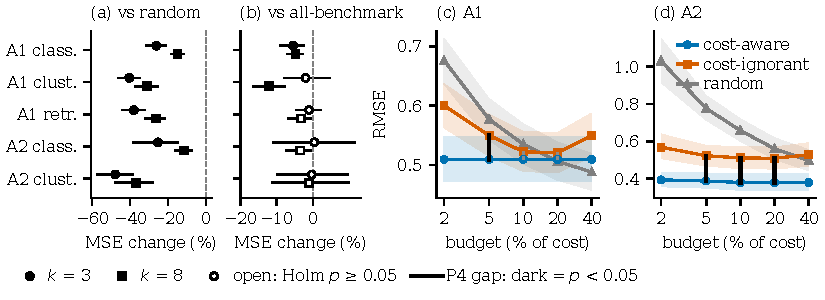
\includegraphics[width=\textwidth]{figures/f3.pdf}
\caption{Groups of tasks and unequal costs. (a, b) Group-targeted A-optimal selection minus random choice (a) and minus the all-benchmark complement-error greedy (b): relative change in group MSE (\%) at $k=3$ (circles) and $k=8$ (squares), 95\% intervals over held-out models; filled: Holm $p<0.05$ over the 20 declared tests. Class., clust., retr.: classification, clustering, retrieval tasks; A1, A2: MTEB-A1, MTEB-A2. (c, d) RMSE against the budget, the share of the summed median evaluation time of all benchmarks, for cost-aware and cost-ignorant A-optimal selection and random choice (bands: 95\%); segments join the two A-optimal choices (dark: Holm $p<0.05$ over six tests; grey dotted: not significant). Curves are evaluated on the $k$ grid; the cost-aware choice is the grid maximum for budgets above $1.7\%$ (A1) and $7\%$ (A2) of the total, so its curve is flat. Five repetitions.}
\label{fig:f3}
\end{figure}

\section{Inference rules at a fixed selection}
\label{app:rules}
\begin{figure}[h]
\centering
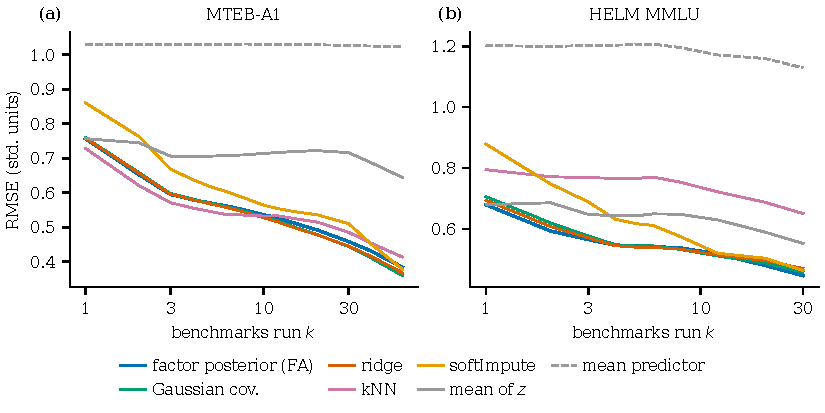
\includegraphics[width=\textwidth]{figures/f6_rules.pdf}
\caption{RMSE against $k$ for six inference rules and the history-mean predictor with the selection fixed (complement-error greedy$^\dagger$), on MTEB-A1 and HELM MMLU: factor posterior, Gaussian covariance conditioning with a shrunk covariance, ridge, kNN, softImpute and mean of the latent scores.}
\end{figure}

\section{Forecast against the size of the history}
\label{app:history}
Varying the history size $M$ (25 test models with their families excluded from the history, 10 repetitions) shows where this stops holding.
On MTEB the forecast is optimistic at every $M$ and the median absolute gap falls with $M$: on A1 $37$, $29$, $21$, $21$ and $18\%$ at $M=20$, $30$, $45$, $60$ and $78$ (within $20\%$ in $23\%$ of the $(M,k)$ cells), on A2 $79\%$ at $M=20$ and $17$--$22\%$ for $M\ge45$.
The selected rank is within 2 of the predicted one only when the history is nearly the whole matrix (A1: $0$, $0$, $10$, $40$ and $100\%$ of repetitions at the same $M$), whereas on the Open LLM Leaderboard matrices ($N=6$ and $40$, $M$ up to $2000$) the median gap is at most $1.2\%$ and $3.4\%$ at $M\ge500$ and the rank is within 2 in every repetition from $M=500$: the correction helps when $M$ is large against $N$ and under-resolves the rank when it is not.

\section{Unseen organisations and simple alternatives}
\label{app:fam}
The held-out models of a random fold share an organisation with models of the history, so the selection gain of Section~\ref{sec:experiments} may partly be an in-distribution effect.
We repeat the MTEB comparisons with the folds made of whole organisations (history without any test organisation) and resample organisations rather than models in the bootstrap; A1 and A2 use five repetitions, B three.
Table~\ref{tab:fam} gives the relative change in MSE of the comparisons of the primary family that involve random choice, and of two simple alternatives that we added after the pilot and did not include in the declared family: forward regression and $k$-medoids on the benchmark correlation.
Table~\ref{tab:famrmse} gives the RMSE.
The Holm correction is over the 15 tests of each matrix and regime and not over the family of Table~\ref{tab:t2}, so signs and significance, not $p$-values, are comparable.
\begin{table}[h]
\centering\scriptsize\setlength{\tabcolsep}{3pt}
\begin{tabular}{@{}ll@{\hspace{9pt}}rrr@{\hspace{9pt}}rrr@{\hspace{9pt}}rrr@{\hspace{9pt}}rrr@{}}
\toprule
& & \multicolumn{3}{c}{A-opt.} & \multicolumn{3}{c}{compl.\,$\dagger$} & \multicolumn{3}{c}{compl.\,$\dagger$} & \multicolumn{3}{c}{compl.\,$\dagger$} \\
& & \multicolumn{3}{c}{vs random} & \multicolumn{3}{c}{vs random} & \multicolumn{3}{c}{vs fwd. regr.} & \multicolumn{3}{c}{vs $k$-medoids} \\
\cmidrule(lr){3-5} \cmidrule(lr){6-8} \cmidrule(lr){9-11} \cmidrule(lr){12-14}
& & 3 & 8 & 20 & 3 & 8 & 20 & 3 & 8 & 20 & 3 & 8 & 20 \\
\midrule
A1 & random folds & \textbf{$-$28} & \textbf{$-$15} & \textbf{$-$3} & \textbf{$-$28} & \textbf{$-$15} & \textbf{$-$15} & $-$1 & $-$2 & \textbf{$-$6} & $+$3 & $-$2 & \textbf{$-$9} \\
 & held-out organisations & \textbf{$-$27} & \textbf{$-$11} & $-$2 & \textbf{$-$27} & \textbf{$-$12} & \textbf{$-$14} & $-$3 & $-$2 & $-$7 & 0 & $-$2 & \textbf{$-$9} \\
\addlinespace[2pt]
A2 & random folds & \textbf{$-$20} & $-$3 & \textbf{$+$52} & \textbf{$-$20} & \textbf{$-$32} & \textbf{$-$50} & $+$1 & \textbf{$-$5} & $-$4 & $+$2 & \textbf{$-$18} & \textbf{$-$37} \\
 & held-out organisations & $-$4 & $+$16 & \textbf{$+$62} & $-$4 & \textbf{$-$77} & \textbf{$-$85} & $-$1 & $-$79 & $-$4 & $+$3 & \textbf{$-$19} & \textbf{$-$38} \\
 & held-out, without one organisation$\,\ddagger$ & \textbf{$-$23} & 0 & \textbf{$+$49} & \textbf{$-$23} & \textbf{$-$24} & \textbf{$-$49} & $-$1 & $-$1 & $-$3 & $+$1 & \textbf{$-$12} & \textbf{$-$30} \\
\addlinespace[2pt]
B & random folds & \textbf{$-$22} & $-$2 & \textbf{$+$14} & \textbf{$-$22} & $-$3 & \textbf{$-$15} & \textbf{$-$9} & $+$7 & \textbf{$-$13} & $-$1 & \textbf{$+$5} & $-$16 \\
 & held-out organisations & \textbf{$-$13} & $+$1 & \textbf{$+$19} & \textbf{$-$12} & 0 & $+$8 & $-$1 & $+$2 & $-$2 & $+$2 & \textbf{$+$6} & $+$4 \\
\bottomrule
\end{tabular}

\caption{Relative change in held-out MSE (\%) at $k=3$, $8$, $20$, first named minus second (negative: first is better), by organisation bootstrap; \textbf{bold}: Holm-adjusted $p<0.05$ over 15 tests. compl.\,$\dagger$: complement-error greedy; each change is divided by the mean MSE of the second selector in the full sample, so an interval end below $-100\%$ is possible and is not an error reduced by more than all of it. The last two comparisons are exploratory. On A2 with held-out organisations the scale is an MSE dominated by one organisation, so the large magnitudes of that row ($-77$, $-79$) mark the tail rather than an effect. $^\ddagger$ The organisation \texttt{codefuse-ai} (8 models, 64\% of the mean-predictor MSE under held-out folds) removed after the fact. Intervals: \texttt{code/results/FAM/TABLES.md}.}
\label{tab:fam}
\end{table}
\begin{table}[h]
\centering\scriptsize\setlength{\tabcolsep}{3pt}
\begin{tabular}{@{}ll@{\hspace{9pt}}rrr@{\hspace{9pt}}rrr@{\hspace{9pt}}rrr@{}}
\toprule
& & \multicolumn{3}{c}{random} & \multicolumn{3}{c}{A-optimal} & \multicolumn{3}{c}{compl.\,$\dagger$} \\
\cmidrule(lr){3-5} \cmidrule(lr){6-8} \cmidrule(lr){9-11}
& & 3 & 8 & 20 & 3 & 8 & 20 & 3 & 8 & 20 \\
\midrule
A1 & random folds & 0.70 & 0.59 & 0.53 & 0.60 & 0.55 & 0.52 & 0.60 & 0.55 & 0.49 \\
 & held-out organisations & 0.74 & 0.64 & 0.59 & 0.63 & 0.60 & 0.58 & 0.63 & 0.60 & 0.54 \\
\addlinespace[2pt]
A2 & random folds & 0.63 & 0.52 & 0.47 & 0.56 & 0.51 & 0.58 & 0.56 & 0.43 & 0.33 \\
 & held-out organisations & 1.22 & 1.16 & 1.13 & 1.20 & 1.25 & 1.43 & 1.20 & 0.56 & 0.43 \\
 & held-out, without one organisation$\,\ddagger$ & 0.63 & 0.54 & 0.49 & 0.56 & 0.54 & 0.60 & 0.55 & 0.47 & 0.35 \\
\addlinespace[2pt]
B & random folds & 0.79 & 0.70 & 0.67 & 0.70 & 0.70 & 0.72 & 0.70 & 0.69 & 0.62 \\
 & held-out organisations & 1.08 & 1.00 & 0.96 & 1.01 & 1.00 & 1.05 & 1.01 & 1.00 & 1.00 \\
\bottomrule
\end{tabular}

\caption{RMSE in standardised units at $k=3$, $8$, $20$ with factor inference, random folds and folds of held-out organisations; compl.\,$\dagger$: complement-error greedy; $\ddagger$ as in Table~\ref{tab:fam}.}
\label{tab:famrmse}
\end{table}
For A1 the held-out organisations leave every direction unchanged; only the small gain of the A-optimal criterion at $k=20$ ($-3\%$ with random folds, $-2\%$ with held-out organisations) is no longer significant.
On A2 one organisation (\texttt{codefuse-ai}) carries 64\% of the mean-predictor error under held-out folds, and the RMSE over all held-out models exceeds 1 at $k=3$ for every selector; the A-optimal criterion is then no better than random choice at $k=3$ and $8$ and $62\%$ worse at $k=20$, whereas the complement-error greedy is better than random at $k=8$ and $20$, with intervals wide because of that tail.
Without that organisation the picture of random folds returns (the row marked $\ddagger$).
On B the gain of the complement-error greedy over random choice at $k=3$ holds ($-12\%$) and at $k=20$ it is a tie ($+8\%$, not significant) against $-15\%$ with random folds.
Resampling organisations widens the intervals of the paired differences by a median of $17\%$ (A1), $18\%$ (A2) and $38\%$ (B) and changes no decision of Table~\ref{tab:t2}.
Against the simple alternatives the complement-error greedy is never worse on A1 and A2 and better than $k$-medoids at $k=20$ ($-9\%$ and $-37\%$); on B it is worse than $k$-medoids at $k=8$ ($+5\%$ with random folds, $+6\%$ with held-out organisations, both significant) and not better than forward regression ($+7\%$, not significant).

\section{Shift}
\label{app:shift}
\begin{figure}[h]
\centering
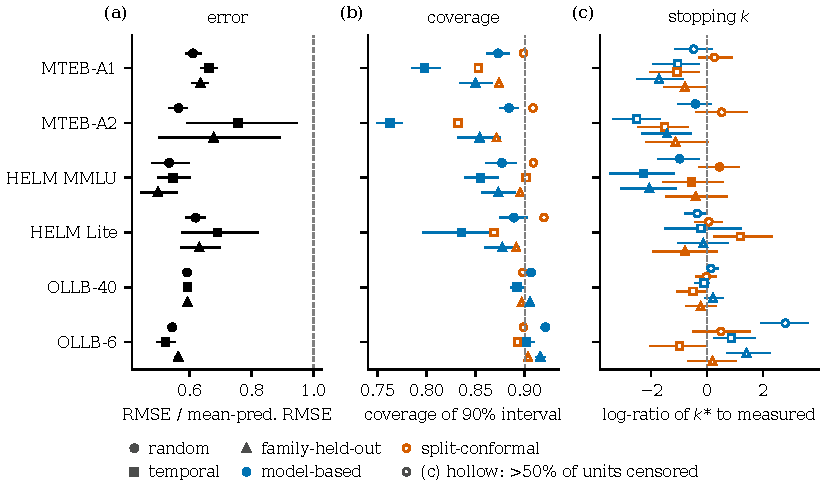
\includegraphics[width=\textwidth]{figures/f5.pdf}
\caption{Shift, A-optimal selection with factor inference, $k=3$ (the largest $k$ every matrix has). Markers: split. (a) RMSE over the mean-predictor RMSE. (b) Coverage of the nominal 90\% interval, model-based and split-conformal. (c) Error of the stopping $k$ (log$_2$ of the rule's $k^\ast$ over the measured $k^\ast$; tolerance 0.5); hollow markers: more than half of the units never reach the tolerance on the grid.}
\label{fig:f5}
\end{figure}
Under temporal splits the model-based intervals cover $0.76$ (A2) and $0.80$ (A1) of the scores at $k=3$, under family-held-out splits $0.85$, and on the generative-LLM matrices within $0.02$--$0.06$ of $0.90$ (panel b); split-conformal intervals cover $0.83$ and $0.85$ under temporal shift on MTEB.
The error relative to the mean predictor rises under temporal shift on MTEB and not on the Open LLM Leaderboard matrices (panel a).
The stopping $k$ of neither rule is uniformly closer to the measured one (panel c).

\section{Reproducing the results}
\label{app:repro}
All experiments run on CPU only.
The supplementary material contains the data extraction with the pinned versions of Appendix~\ref{app:data}, the analysis code (selectors, factor analysis with missing data, the protocol of Section~\ref{sec:setting}, the theory formulas), one driver script per experiment with its seeds, the result files from which every figure and table is drawn, and the scripts that draw them.
Jobs ran on two CPU cores each of a shared Intel Xeon Gold 6230 host, with 0.1--0.8 GB of memory, Python 3.11 with NumPy 2.4, SciPy 1.17, pandas 3.0 and scikit-learn 1.9, one BLAS thread per process; repetition $r$ seeds the split and every random draw with $r$.
Fitting the models of one repetition (five folds) takes a median of 3.5 minutes on A2 and 7.8 minutes on A1; the whole ten-repetition runs took about 33 minutes (A2) and 75 minutes (A1) of wall-clock time on the loaded host.
The leakage ablation takes 3 minutes (A1) and 1 minute (A2) per repetition, and the factor-model fits of the generative-LLM leaderboards 1 to 3 minutes per repetition, 26 and 36 minutes for the two Open LLM Leaderboard matrices.
The nonlinear imputers of Section~\ref{sec:experiments} dominate the cost on A1 (more than two hours for five repetitions on the full grid).


\section*{NeurIPS Paper Checklist}




\begin{enumerate}

\item {\bf Claims}
    \item[] Question: Do the main claims made in the abstract and introduction accurately reflect the paper's contributions and scope?
    \item[] Answer: \answerYes{} % Replace by \answerYes{}, \answerNo{}, or \answerNA{}.
    \item[] Justification: The abstract and Section~\ref{sec:intro} state the problem, the three contributions and the results; Sections~\ref{sec:experiments} and \ref{sec:discussion} give the evidence and the limits, including the claims that failed (finite-history forecast, factor-posterior accuracy).
    \item[] Guidelines:
    \begin{itemize}
        \item The answer \answerNA{} means that the abstract and introduction do not include the claims made in the paper.
        \item The abstract and/or introduction should clearly state the claims made, including the contributions made in the paper and important assumptions and limitations. A \answerNo{} or \answerNA{} answer to this question will not be perceived well by the reviewers. 
        \item The claims made should match theoretical and experimental results, and reflect how much the results can be expected to generalize to other settings. 
        \item It is fine to include aspirational goals as motivation as long as it is clear that these goals are not attained by the paper. 
    \end{itemize}

\item {\bf Limitations}
    \item[] Question: Does the paper discuss the limitations of the work performed by the authors?
    \item[] Answer: \answerYes{} % Replace by \answerYes{}, \answerNo{}, or \answerNA{}.
    \item[] Justification: Section~\ref{sec:discussion} lists the limits: optimistic forecast, post-pilot selector, shift, size of the generative-LLM matrices, data licences.
    \item[] Guidelines:
    \begin{itemize}
        \item The answer \answerNA{} means that the paper has no limitation while the answer \answerNo{} means that the paper has limitations, but those are not discussed in the paper. 
        \item The authors are encouraged to create a separate ``Limitations'' section in their paper.
        \item The paper should point out any strong assumptions and how robust the results are to violations of these assumptions (e.g., independence assumptions, noiseless settings, model well-specification, asymptotic approximations only holding locally). The authors should reflect on how these assumptions might be violated in practice and what the implications would be.
        \item The authors should reflect on the scope of the claims made, e.g., if the approach was only tested on a few datasets or with a few runs. In general, empirical results often depend on implicit assumptions, which should be articulated.
        \item The authors should reflect on the factors that influence the performance of the approach. For example, a facial recognition algorithm may perform poorly when image resolution is low or images are taken in low lighting. Or a speech-to-text system might not be used reliably to provide closed captions for online lectures because it fails to handle technical jargon.
        \item The authors should discuss the computational efficiency of the proposed algorithms and how they scale with dataset size.
        \item If applicable, the authors should discuss possible limitations of their approach to address problems of privacy and fairness.
        \item While the authors might fear that complete honesty about limitations might be used by reviewers as grounds for rejection, a worse outcome might be that reviewers discover limitations that aren't acknowledged in the paper. The authors should use their best judgment and recognize that individual actions in favor of transparency play an important role in developing norms that preserve the integrity of the community. Reviewers will be specifically instructed to not penalize honesty concerning limitations.
    \end{itemize}

\item {\bf Theory assumptions and proofs}
    \item[] Question: For each theoretical result, does the paper provide the full set of assumptions and a complete (and correct) proof?
    \item[] Answer: \answerYes{} % Replace by \answerYes{}, \answerNo{}, or \answerNA{}.
    \item[] Justification: Assumptions are stated with each proposition in Section~\ref{sec:theory}; proofs are in Appendix~\ref{app:proofs}; the finite-history statement is labelled a conjecture and tested in Section~\ref{sec:experiments}.
    \item[] Guidelines:
    \begin{itemize}
        \item The answer \answerNA{} means that the paper does not include theoretical results. 
        \item All the theorems, formulas, and proofs in the paper should be numbered and cross-referenced.
        \item All assumptions should be clearly stated or referenced in the statement of any theorems.
        \item The proofs can either appear in the main paper or the supplemental material, but if they appear in the supplemental material, the authors are encouraged to provide a short proof sketch to provide intuition. 
        \item Inversely, any informal proof provided in the core of the paper should be complemented by formal proofs provided in appendix or supplemental material.
        \item Theorems and Lemmas that the proof relies upon should be properly referenced. 
    \end{itemize}

    \item {\bf Experimental result reproducibility}
    \item[] Question: Does the paper fully disclose all the information needed to reproduce the main experimental results of the paper to the extent that it affects the main claims and/or conclusions of the paper (regardless of whether the code and data are provided or not)?
    \item[] Answer: \answerYes{} % Replace by \answerYes{}, \answerNo{}, or \answerNA{}.
    \item[] Justification: Sections~\ref{sec:setting} and \ref{sec:method} and Appendix~\ref{app:repro} give the protocol, the model, the selectors, the hyper-parameter selection, the data versions and the commands; the code regenerates every result file.
    \item[] Guidelines:
    \begin{itemize}
        \item The answer \answerNA{} means that the paper does not include experiments.
        \item If the paper includes experiments, a \answerNo{} answer to this question will not be perceived well by the reviewers: Making the paper reproducible is important, regardless of whether the code and data are provided or not.
        \item If the contribution is a dataset and\slash or model, the authors should describe the steps taken to make their results reproducible or verifiable. 
        \item Depending on the contribution, reproducibility can be accomplished in various ways. For example, if the contribution is a novel architecture, describing the architecture fully might suffice, or if the contribution is a specific model and empirical evaluation, it may be necessary to either make it possible for others to replicate the model with the same dataset, or provide access to the model. In general. releasing code and data is often one good way to accomplish this, but reproducibility can also be provided via detailed instructions for how to replicate the results, access to a hosted model (e.g., in the case of a large language model), releasing of a model checkpoint, or other means that are appropriate to the research performed.
        \item While NeurIPS does not require releasing code, the conference does require all submissions to provide some reasonable avenue for reproducibility, which may depend on the nature of the contribution. For example
        \begin{enumerate}
            \item If the contribution is primarily a new algorithm, the paper should make it clear how to reproduce that algorithm.
            \item If the contribution is primarily a new model architecture, the paper should describe the architecture clearly and fully.
            \item If the contribution is a new model (e.g., a large language model), then there should either be a way to access this model for reproducing the results or a way to reproduce the model (e.g., with an open-source dataset or instructions for how to construct the dataset).
            \item We recognize that reproducibility may be tricky in some cases, in which case authors are welcome to describe the particular way they provide for reproducibility. In the case of closed-source models, it may be that access to the model is limited in some way (e.g., to registered users), but it should be possible for other researchers to have some path to reproducing or verifying the results.
        \end{enumerate}
    \end{itemize}


\item {\bf Open access to data and code}
    \item[] Question: Does the paper provide open access to the data and code, with sufficient instructions to faithfully reproduce the main experimental results, as described in supplemental material?
    \item[] Answer: \answerYes{} % Replace by \answerYes{}, \answerNo{}, or \answerNA{}.
    \item[] Justification: Code, data extraction with pinned versions and the result files are in the supplementary material; Appendix~\ref{app:repro} says how to rerun them.
    \item[] Guidelines:
    \begin{itemize}
        \item The answer \answerNA{} means that paper does not include experiments requiring code.
        \item Please see the NeurIPS code and data submission guidelines (\url{https://neurips.cc/public/guides/CodeSubmissionPolicy}) for more details.
        \item While we encourage the release of code and data, we understand that this might not be possible, so \answerNo{} is an acceptable answer. Papers cannot be rejected simply for not including code, unless this is central to the contribution (e.g., for a new open-source benchmark).
        \item The instructions should contain the exact command and environment needed to run to reproduce the results. See the NeurIPS code and data submission guidelines (\url{https://neurips.cc/public/guides/CodeSubmissionPolicy}) for more details.
        \item The authors should provide instructions on data access and preparation, including how to access the raw data, preprocessed data, intermediate data, and generated data, etc.
        \item The authors should provide scripts to reproduce all experimental results for the new proposed method and baselines. If only a subset of experiments are reproducible, they should state which ones are omitted from the script and why.
        \item At submission time, to preserve anonymity, the authors should release anonymized versions (if applicable).
        \item Providing as much information as possible in supplemental material (appended to the paper) is recommended, but including URLs to data and code is permitted.
    \end{itemize}


\item {\bf Experimental setting/details}
    \item[] Question: Does the paper specify all the training and test details (e.g., data splits, hyperparameters, how they were chosen, type of optimizer) necessary to understand the results?
    \item[] Answer: \answerYes{} % Replace by \answerYes{}, \answerNo{}, or \answerNA{}.
    \item[] Justification: Section~\ref{sec:setting} and Appendix~\ref{app:repro}: splits, repetitions, hyper-parameter selection inside the history, budgets and tolerances.
    \item[] Guidelines:
    \begin{itemize}
        \item The answer \answerNA{} means that the paper does not include experiments.
        \item The experimental setting should be presented in the core of the paper to a level of detail that is necessary to appreciate the results and make sense of them.
        \item The full details can be provided either with the code, in appendix, or as supplemental material.
    \end{itemize}

\item {\bf Experiment statistical significance}
    \item[] Question: Does the paper report error bars suitably and correctly defined or other appropriate information about the statistical significance of the experiments?
    \item[] Answer: \answerYes{} % Replace by \answerYes{}, \answerNo{}, or \answerNA{}.
    \item[] Justification: Every curve and difference carries a 95\% bootstrap interval over held-out models (the unit of replication); confidence intervals in Table~\ref{tab:t2} are unadjusted and the Holm-adjusted decision is marked.
    \item[] Guidelines:
    \begin{itemize}
        \item The answer \answerNA{} means that the paper does not include experiments.
        \item The authors should answer \answerYes{} if the results are accompanied by error bars, confidence intervals, or statistical significance tests, at least for the experiments that support the main claims of the paper.
        \item The factors of variability that the error bars are capturing should be clearly stated (for example, train/test split, initialization, random drawing of some parameter, or overall run with given experimental conditions).
        \item The method for calculating the error bars should be explained (closed form formula, call to a library function, bootstrap, etc.)
        \item The assumptions made should be given (e.g., Normally distributed errors).
        \item It should be clear whether the error bar is the standard deviation or the standard error of the mean.
        \item It is OK to report 1-sigma error bars, but one should state it. The authors should preferably report a 2-sigma error bar than state that they have a 96\% CI, if the hypothesis of Normality of errors is not verified.
        \item For asymmetric distributions, the authors should be careful not to show in tables or figures symmetric error bars that would yield results that are out of range (e.g., negative error rates).
        \item If error bars are reported in tables or plots, the authors should explain in the text how they were calculated and reference the corresponding figures or tables in the text.
    \end{itemize}

\item {\bf Experiments compute resources}
    \item[] Question: For each experiment, does the paper provide sufficient information on the computer resources (type of compute workers, memory, time of execution) needed to reproduce the experiments?
    \item[] Answer: \answerYes{} % Replace by \answerYes{}, \answerNo{}, or \answerNA{}.
    \item[] Justification: Appendix~\ref{app:repro}: CPU-only runs; hardware and wall-clock time per experiment.
    \item[] Guidelines:
    \begin{itemize}
        \item The answer \answerNA{} means that the paper does not include experiments.
        \item The paper should indicate the type of compute workers CPU or GPU, internal cluster, or cloud provider, including relevant memory and storage.
        \item The paper should provide the amount of compute required for each of the individual experimental runs as well as estimate the total compute. 
        \item The paper should disclose whether the full research project required more compute than the experiments reported in the paper (e.g., preliminary or failed experiments that didn't make it into the paper). 
    \end{itemize}
    
\item {\bf Code of ethics}
    \item[] Question: Does the research conducted in the paper conform, in every respect, with the NeurIPS Code of Ethics \url{https://neurips.cc/public/EthicsGuidelines}?
    \item[] Answer: \answerYes{} % Replace by \answerYes{}, \answerNo{}, or \answerNA{}.
    \item[] Justification: The work uses public score tables only and involves no human subjects or personal data; it conforms to the NeurIPS Code of Ethics.
    \item[] Guidelines:
    \begin{itemize}
        \item The answer \answerNA{} means that the authors have not reviewed the NeurIPS Code of Ethics.
        \item If the authors answer \answerNo, they should explain the special circumstances that require a deviation from the Code of Ethics.
        \item The authors should make sure to preserve anonymity (e.g., if there is a special consideration due to laws or regulations in their jurisdiction).
    \end{itemize}


\item {\bf Broader impacts}
    \item[] Question: Does the paper discuss both potential positive societal impacts and negative societal impacts of the work performed?
    \item[] Answer: \answerNA{} % Replace by \answerYes{}, \answerNo{}, or \answerNA{}.
    \item[] Justification: The work is a methodology for choosing benchmarks on public leaderboards; we see no direct societal impact beyond the general effect of cheaper model evaluation, and note that fewer benchmarks can hide failures on those not run (Section~\ref{sec:discussion}).
    \item[] Guidelines:
    \begin{itemize}
        \item The answer \answerNA{} means that there is no societal impact of the work performed.
        \item If the authors answer \answerNA{} or \answerNo, they should explain why their work has no societal impact or why the paper does not address societal impact.
        \item Examples of negative societal impacts include potential malicious or unintended uses (e.g., disinformation, generating fake profiles, surveillance), fairness considerations (e.g., deployment of technologies that could make decisions that unfairly impact specific groups), privacy considerations, and security considerations.
        \item The conference expects that many papers will be foundational research and not tied to particular applications, let alone deployments. However, if there is a direct path to any negative applications, the authors should point it out. For example, it is legitimate to point out that an improvement in the quality of generative models could be used to generate Deepfakes for disinformation. On the other hand, it is not needed to point out that a generic algorithm for optimizing neural networks could enable people to train models that generate Deepfakes faster.
        \item The authors should consider possible harms that could arise when the technology is being used as intended and functioning correctly, harms that could arise when the technology is being used as intended but gives incorrect results, and harms following from (intentional or unintentional) misuse of the technology.
        \item If there are negative societal impacts, the authors could also discuss possible mitigation strategies (e.g., gated release of models, providing defenses in addition to attacks, mechanisms for monitoring misuse, mechanisms to monitor how a system learns from feedback over time, improving the efficiency and accessibility of ML).
    \end{itemize}
    
\item {\bf Safeguards}
    \item[] Question: Does the paper describe safeguards that have been put in place for responsible release of data or models that have a high risk for misuse (e.g., pre-trained language models, image generators, or scraped datasets)?
    \item[] Answer: \answerNA{} % Replace by \answerYes{}, \answerNo{}, or \answerNA{}.
    \item[] Justification: No model or scraped data with misuse risk is released.
    \item[] Guidelines:
    \begin{itemize}
        \item The answer \answerNA{} means that the paper poses no such risks.
        \item Released models that have a high risk for misuse or dual-use should be released with necessary safeguards to allow for controlled use of the model, for example by requiring that users adhere to usage guidelines or restrictions to access the model or implementing safety filters. 
        \item Datasets that have been scraped from the Internet could pose safety risks. The authors should describe how they avoided releasing unsafe images.
        \item We recognize that providing effective safeguards is challenging, and many papers do not require this, but we encourage authors to take this into account and make a best faith effort.
    \end{itemize}

\item {\bf Licenses for existing assets}
    \item[] Question: Are the creators or original owners of assets (e.g., code, data, models), used in the paper, properly credited and are the license and terms of use explicitly mentioned and properly respected?
    \item[] Answer: \answerYes{} % Replace by \answerYes{}, \answerNo{}, or \answerNA{}.
    \item[] Justification: Sources, versions and licences are in Appendix~\ref{app:data}; where a publisher states no licence we say so.
    \item[] Guidelines:
    \begin{itemize}
        \item The answer \answerNA{} means that the paper does not use existing assets.
        \item The authors should cite the original paper that produced the code package or dataset.
        \item The authors should state which version of the asset is used and, if possible, include a URL.
        \item The name of the license (e.g., CC-BY 4.0) should be included for each asset.
        \item For scraped data from a particular source (e.g., website), the copyright and terms of service of that source should be provided.
        \item If assets are released, the license, copyright information, and terms of use in the package should be provided. For popular datasets, \url{paperswithcode.com/datasets} has curated licenses for some datasets. Their licensing guide can help determine the license of a dataset.
        \item For existing datasets that are re-packaged, both the original license and the license of the derived asset (if it has changed) should be provided.
        \item If this information is not available online, the authors are encouraged to reach out to the asset's creators.
    \end{itemize}

\item {\bf New assets}
    \item[] Question: Are new assets introduced in the paper well documented and is the documentation provided alongside the assets?
    \item[] Answer: \answerYes{} % Replace by \answerYes{}, \answerNo{}, or \answerNA{}.
    \item[] Justification: The released code and processed matrices are documented in the supplementary material; the processed matrices keep the licence of their sources.
    \item[] Guidelines:
    \begin{itemize}
        \item The answer \answerNA{} means that the paper does not release new assets.
        \item Researchers should communicate the details of the dataset\slash code\slash model as part of their submissions via structured templates. This includes details about training, license, limitations, etc. 
        \item The paper should discuss whether and how consent was obtained from people whose asset is used.
        \item At submission time, remember to anonymize your assets (if applicable). You can either create an anonymized URL or include an anonymized zip file.
    \end{itemize}

\item {\bf Crowdsourcing and research with human subjects}
    \item[] Question: For crowdsourcing experiments and research with human subjects, does the paper include the full text of instructions given to participants and screenshots, if applicable, as well as details about compensation (if any)? 
    \item[] Answer: \answerNA{} % Replace by \answerYes{}, \answerNo{}, or \answerNA{}.
    \item[] Justification: No crowdsourcing or human subjects.
    \item[] Guidelines:
    \begin{itemize}
        \item The answer \answerNA{} means that the paper does not involve crowdsourcing nor research with human subjects.
        \item Including this information in the supplemental material is fine, but if the main contribution of the paper involves human subjects, then as much detail as possible should be included in the main paper. 
        \item According to the NeurIPS Code of Ethics, workers involved in data collection, curation, or other labor should be paid at least the minimum wage in the country of the data collector. 
    \end{itemize}

\item {\bf Institutional review board (IRB) approvals or equivalent for research with human subjects}
    \item[] Question: Does the paper describe potential risks incurred by study participants, whether such risks were disclosed to the subjects, and whether Institutional Review Board (IRB) approvals (or an equivalent approval/review based on the requirements of your country or institution) were obtained?
    \item[] Answer: \answerNA{} % Replace by \answerYes{}, \answerNo{}, or \answerNA{}.
    \item[] Justification: No human subjects.
    \item[] Guidelines:
    \begin{itemize}
        \item The answer \answerNA{} means that the paper does not involve crowdsourcing nor research with human subjects.
        \item Depending on the country in which research is conducted, IRB approval (or equivalent) may be required for any human subjects research. If you obtained IRB approval, you should clearly state this in the paper. 
        \item We recognize that the procedures for this may vary significantly between institutions and locations, and we expect authors to adhere to the NeurIPS Code of Ethics and the guidelines for their institution. 
        \item For initial submissions, do not include any information that would break anonymity (if applicable), such as the institution conducting the review.
    \end{itemize}

\item {\bf Declaration of LLM usage}
    \item[] Question: Does the paper describe the usage of LLMs if it is an important, original, or non-standard component of the core methods in this research? Note that if the LLM is used only for writing, editing, or formatting purposes and does \emph{not} impact the core methodology, scientific rigor, or originality of the research, declaration is not required.
    %this research? 
    \item[] Answer: \answerNA{} % Replace by \answerYes{}, \answerNo{}, or \answerNA{}.
    \item[] Justification: LLMs are the subjects whose scores are modelled; they are not a component of the method.
    \item[] Guidelines:
    \begin{itemize}
        \item The answer \answerNA{} means that the core method development in this research does not involve LLMs as any important, original, or non-standard components.
        \item Please refer to our LLM policy in the NeurIPS handbook for what should or should not be described.
    \end{itemize}

\end{enumerate}
\end{document}
